\chapter{系统详细设计及实现}

本章从代码实现角度说明 CulCloud 的核心模块。系统前端主要位于 \texttt{file-cloud-frontend/src/views/}，统一 API 调用位于 \texttt{file-cloud-frontend/src/services/api.ts}；后端主入口位于 \texttt{backend/app/main.py}，业务路由位于 \texttt{backend/app/routers/}，领域服务位于 \texttt{backend/app/services/}。图 \ref{fig:chap05-component-design} 给出了详细设计组件协作关系，为后续模块说明提供总览。

\begin{figure}[H]
  \centering
  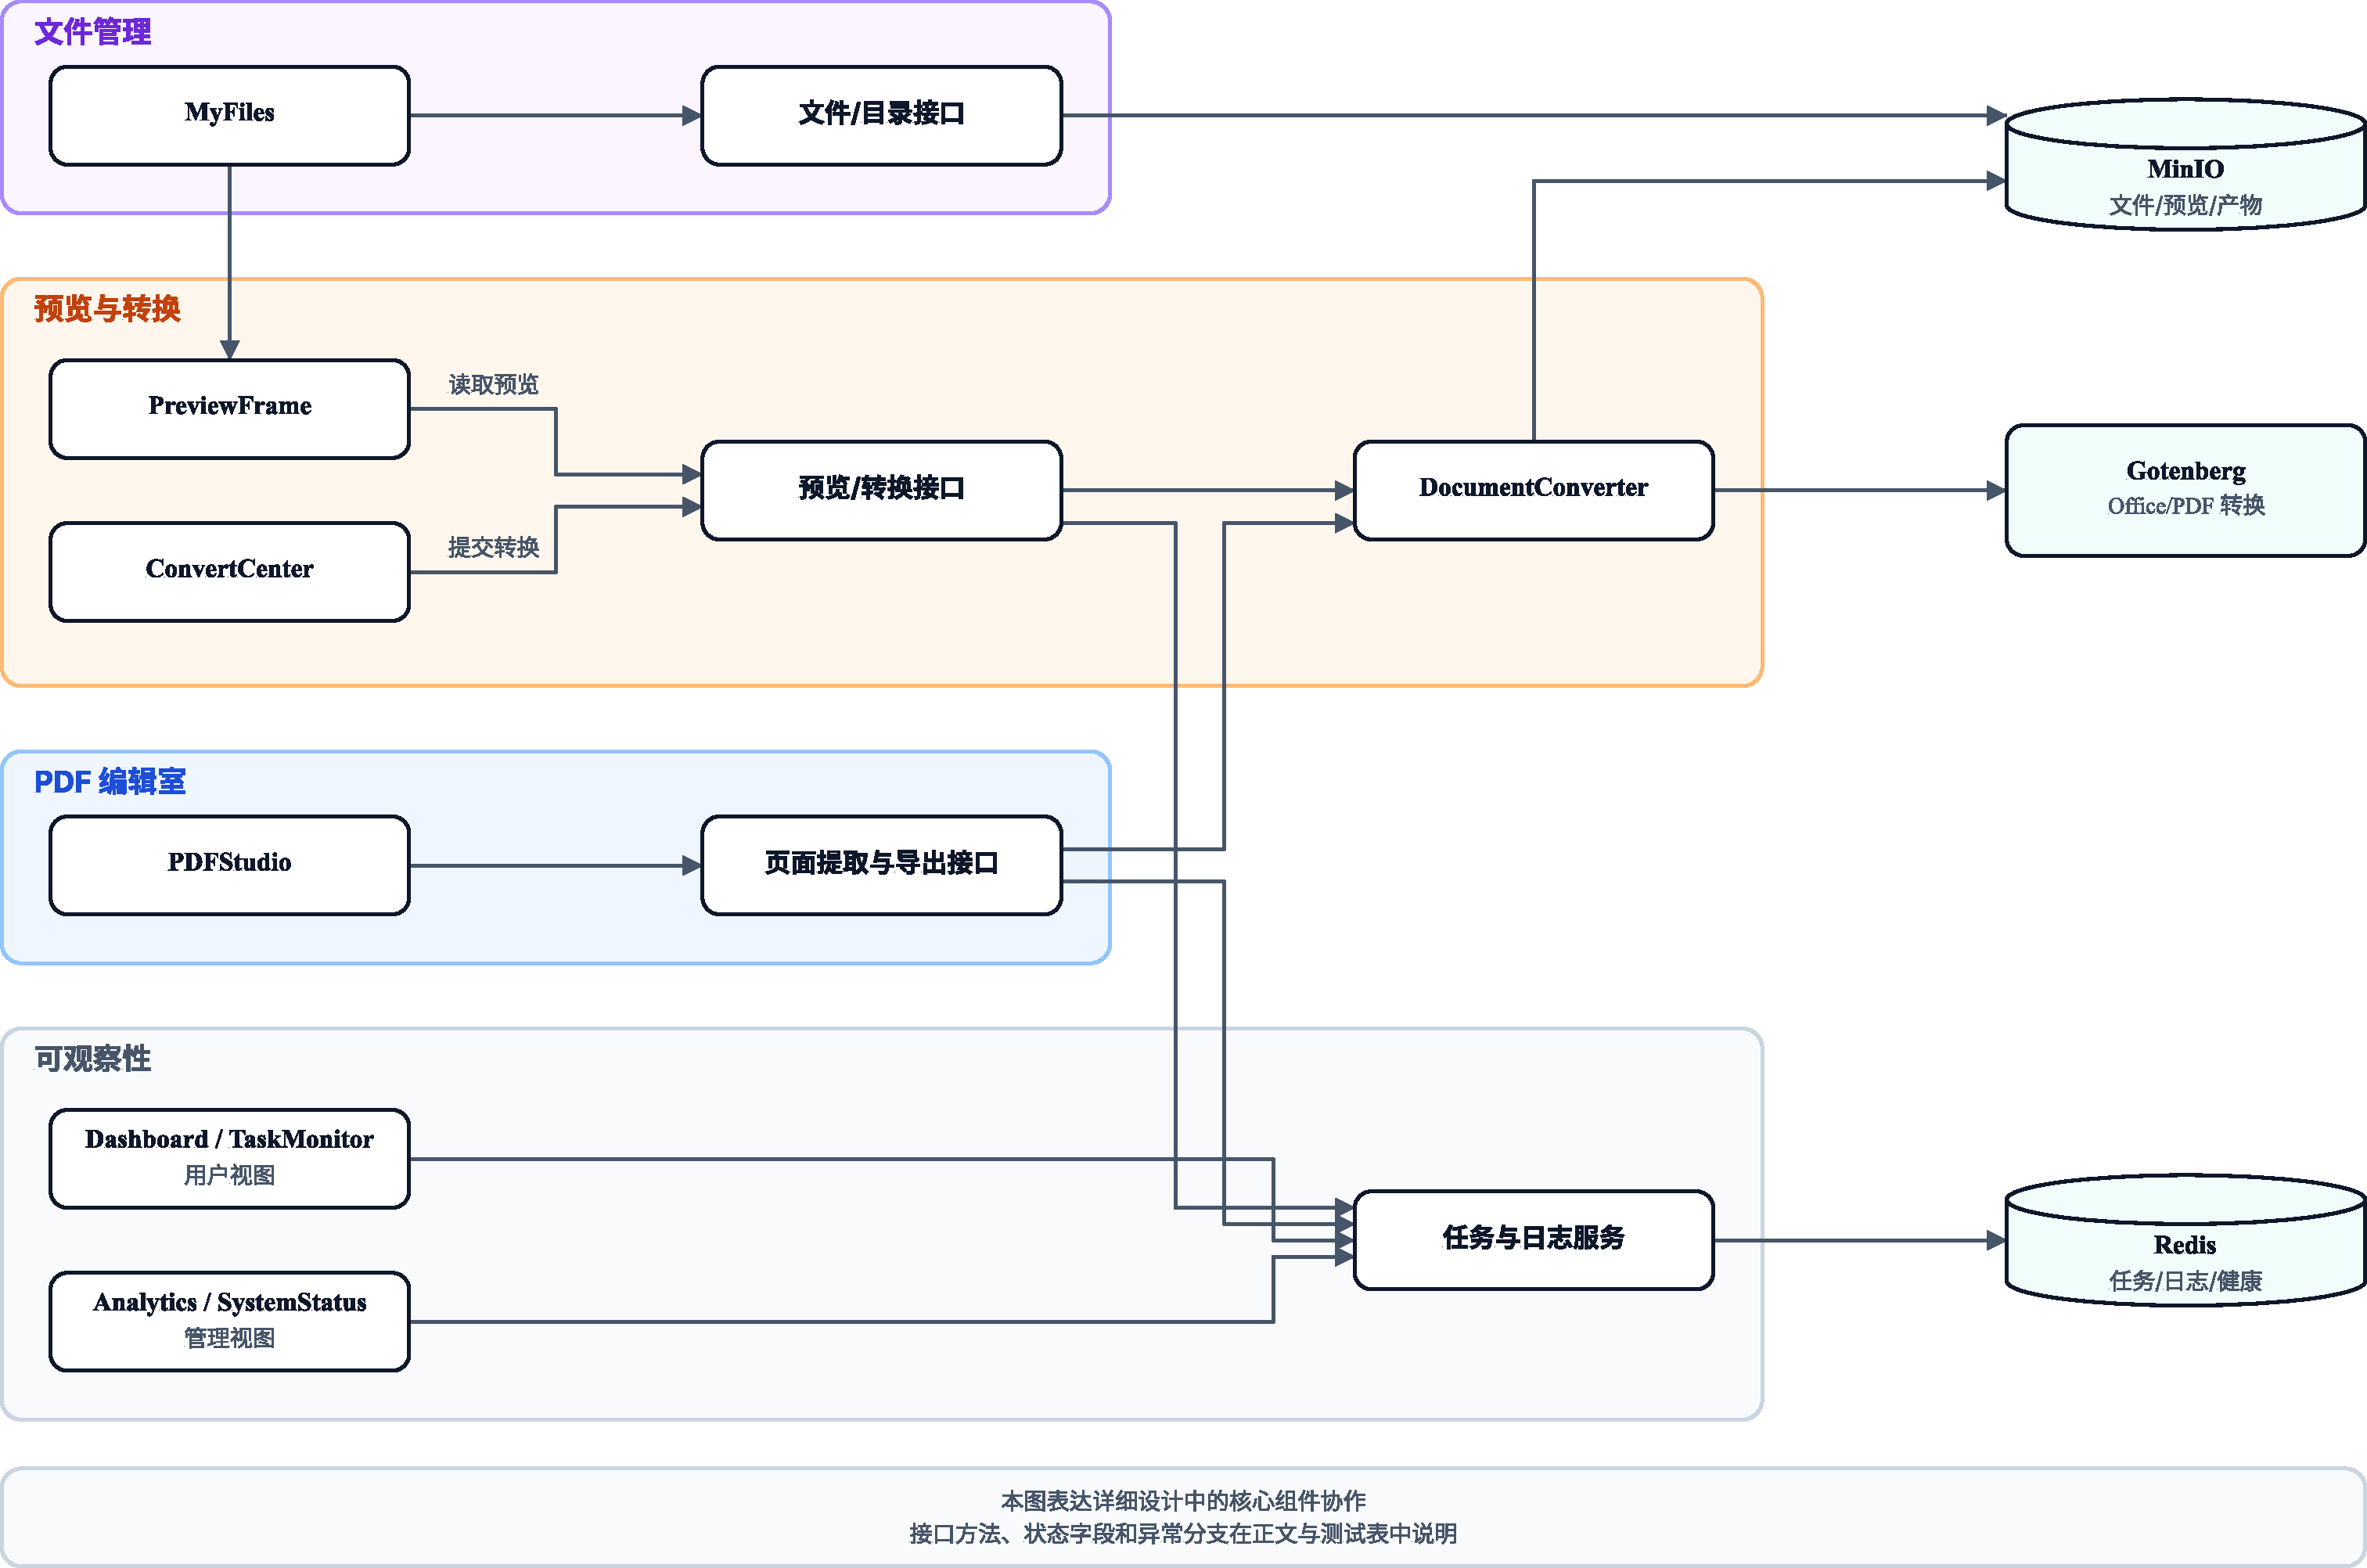
\includegraphics[width=0.96\textwidth,height=0.55\textheight,keepaspectratio]{figures-pdf/fig15-详细设计组件协作.pdf}
  \caption{核心功能详细设计组件协作图}
  \label{fig:chap05-component-design}
\end{figure}

\section{个人首页模块的实现}

\subsection{真实指标聚合}

个人首页由 \texttt{Dashboard.tsx} 实现，主要展示文件数量、存储空间、近期任务和失败提醒。该模块不使用静态计数，而是通过 \texttt{services/api.ts} 中的 \texttt{listFiles}、\texttt{listTasks}、\texttt{getTaskStats} 等函数读取后端数据。文件数量和容量来自 \texttt{/api/v1/files} 返回的 MinIO 对象元数据，任务成功和失败数量来自 Redis 任务索引。当前设计的关键点是让首页指标跟随真实文件处理行为变化，避免用户端完成转换后首页仍显示旧状态。

实现上，首页指标不直接读取浏览器缓存，而是把接口返回作为唯一可信来源。当前文件总量由递归文件列表聚合得到，任务数据由 \texttt{/api/v1/tasks/stats} 提供，近期失败可进一步通过 \texttt{/api/v1/tasks/recent-failures} 获取。这样处理的好处是页面刷新、前端重启或切换端侧后，指标仍能从后端状态恢复；缺点是首页依赖后端服务可用性，因此前端需要为接口异常提供明确提示，而不能默默显示零值。

\subsection{失败原因回溯}

失败任务提示依赖 \texttt{task\_queue.py} 和 \texttt{task\_tracker.py} 中的状态写入逻辑。当转换或 PDF 导出失败时，后端将错误原因写入任务对象的 \texttt{error} 字段，并通过任务接口返回给前端。前端在任务提示或历史列表中读取该字段，使用户能够区分格式不支持、文件损坏、转换服务不可用等不同故障来源。该实现使“失败计数”和“失败原因”具有同一后端来源。

从现场说明角度看，首页模块可以概括为“指标聚合层”：它本身不处理文件，也不执行转换，而是把文件管理、转换任务和异常状态聚合到一个用户可读入口。该设计降低了用户在多模块之间寻找结果的成本，也让后续管理端能够复用同一批任务与日志数据。

\section{我的文件模块的实现}

\subsection{上传、目录与类型分类}

我的文件模块由 \texttt{MyFiles.tsx} 实现，后端对应 \texttt{files.py} 与 \texttt{folders.py}。上传时，前端调用 \texttt{uploadFile(file,\{prefix,relativePath\})}，后端执行路径清洗、对象命名和 MinIO 写入，并通过 \texttt{log\_event} 记录文件上传事件。目录能力并不依赖传统关系数据库表，而是使用对象名前缀和 \texttt{.keep} 空对象表达。前端通过 \texttt{currentPrefix} 维护当前目录，文件类型由扩展名映射到 PDF、文档、表格、PPT、图片、文本、压缩包和其他类型。

该模块的关键实现边界在于：前端只负责组织交互状态和展示分类，不直接操作对象存储；对象命名、路径合法性和文件内容写入均在后端完成。后端 \texttt{\_sanitize\_path} 会拒绝包含危险路径片段的输入，避免用户通过相对路径影响系统目录。文件上传完成后，前端重新拉取列表而不是本地拼接文件项，保证显示内容与 MinIO 中的实际对象保持一致。

上传后的容量展示采用对象大小聚合结果，与第 3 章式 \ref{eq:req-storage-size} 保持一致。前端只展示接口返回的文件大小和汇总容量，不把本地选择文件时的临时大小作为最终值。这样即使后端对文件名、路径或对象前缀进行了清洗，页面上看到的仍然是对象存储确认后的结果。

\subsection{目录操作与对象移动}

文件移动由 \texttt{moveToFolder} 调用 \texttt{/api/v1/folders/move} 完成。后端路由 \texttt{folders.py} 校验目标目录是否存在，并通过 MinIO 的复制和删除完成对象迁移。对文件夹删除、重命名和移动等操作，系统需要处理前缀递归关系，避免将父目录移动到自身子目录中造成路径循环。表 \ref{tab:chap05-code-map} 汇总了用户端主要模块与后端实现位置。

由于对象存储没有真正的目录表，所有目录操作最终都会落到对象名前缀变化上。系统把“路径前缀”作为目录语义，把“对象名”作为文件唯一定位依据，使文件夹浏览、文件移动和文件下载可以共享同一套对象模型。这种设计简化了数据层，但要求后端在移动和删除时格外注意级联对象范围，避免误删预览缓存或转换产物。

\begin{table}[H]
  \centering
  \small
  \caption{核心模块代码位置与数据链路}
  \label{tab:chap05-code-map}
  \begin{tabularx}{\textwidth}{llXX}
    \toprule
    模块 & 前端位置 & 后端位置 & 主要数据对象 \\
    \midrule
    我的文件 & \texttt{MyFiles} & 文件/目录路由 & MinIO 文件对象、目录前缀 \\
    文件预览 & \texttt{PreviewFrame} & 预览路由与预览服务 & 预览类型、预览缓存 \\
    转换中心 & \texttt{ConvertCenter} & 转换路由与转换服务 & Redis 任务、转换产物 \\
    PDF 编辑室 & \texttt{PDFStudio} & PDF 处理接口与转换服务 & 页面配置、批注对象、PDF 产物 \\
    管理驾驶舱 & \texttt{Analytics} & 任务、日志、健康与分析接口 & 实时指标、历史分析样本 \\
    \bottomrule
  \end{tabularx}
\end{table}

图 \ref{fig:chap05-file-manual-group} 展示了文件管理模块的运行结果。左图为根目录与文件夹视图，右图为上传后的文件列表和类型筛选视图。可以看到，文件对象进入列表后保留名称、大小、更新时间和格式标识，说明前端列表与 MinIO 对象元数据已经建立映射。

\begin{figure}[H]
  \centering
  \begin{subfigure}{0.48\textwidth}
    \centering
    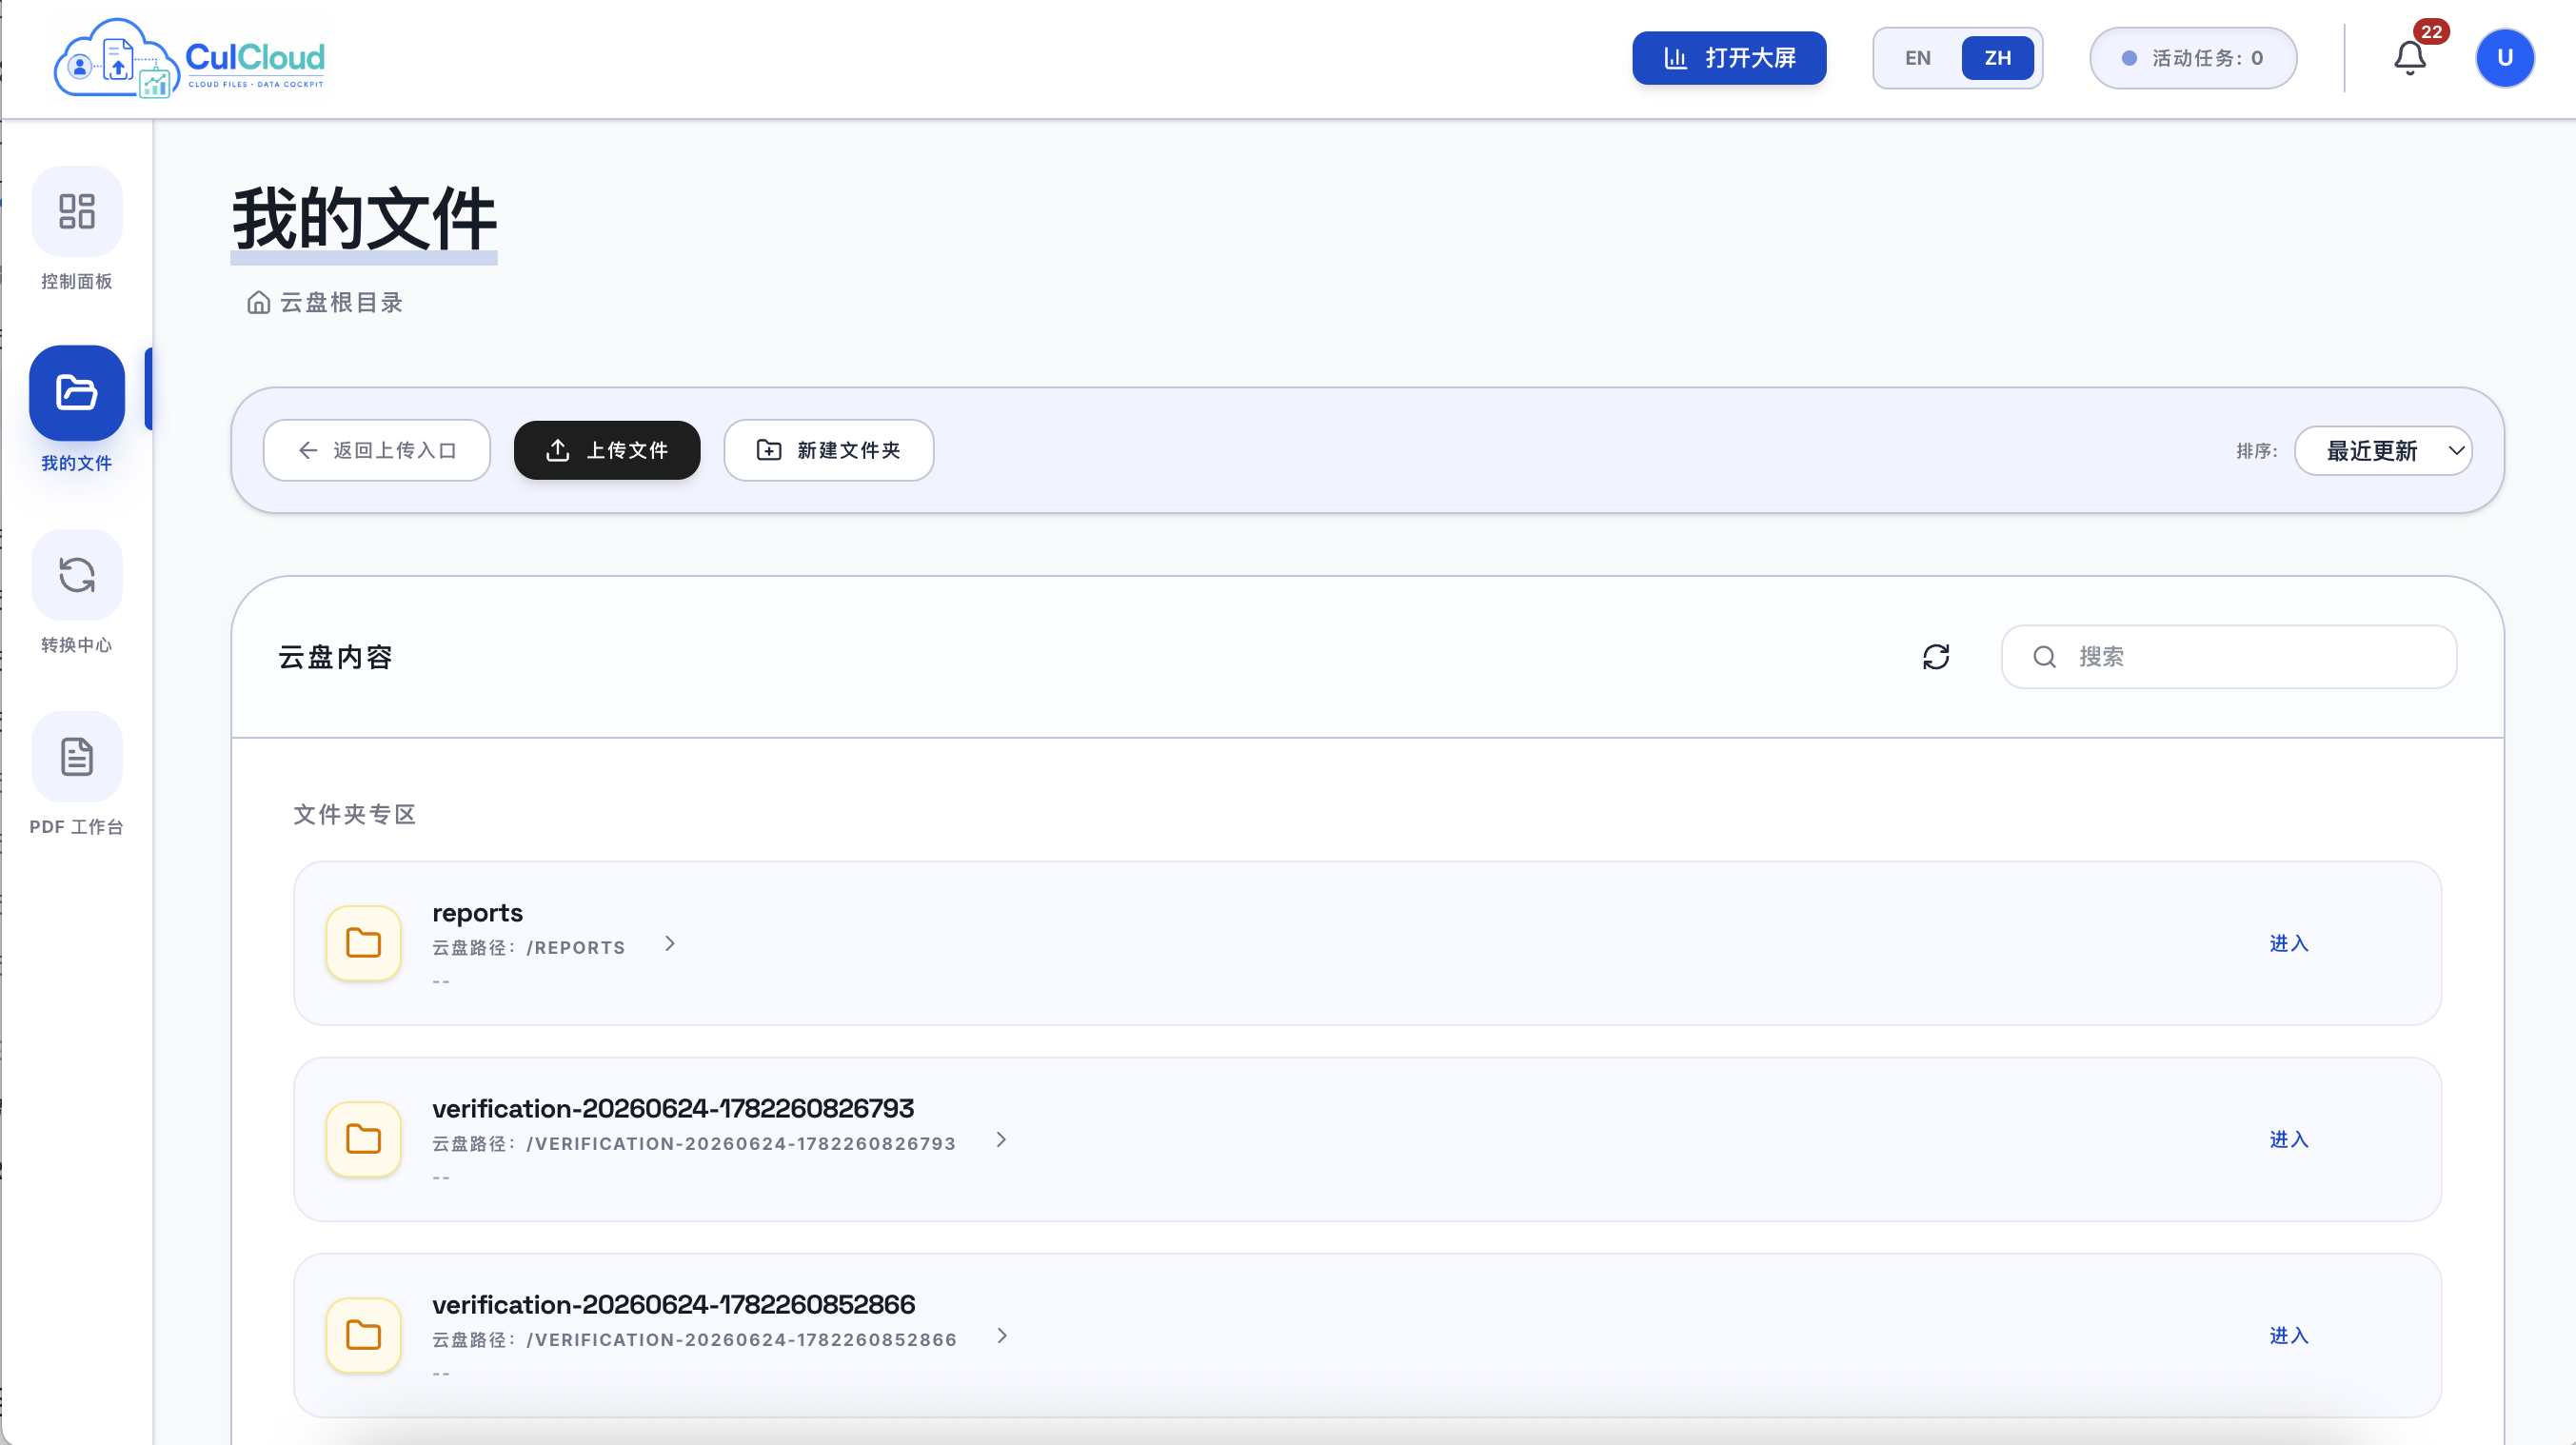
\includegraphics[width=\linewidth,height=0.25\textheight,keepaspectratio]{figures-png/ui/manual/fig05-manual-01-file-folders-root.png}
    \caption{目录与文件夹视图}
  \end{subfigure}
  \hfill
  \begin{subfigure}{0.48\textwidth}
    \centering
    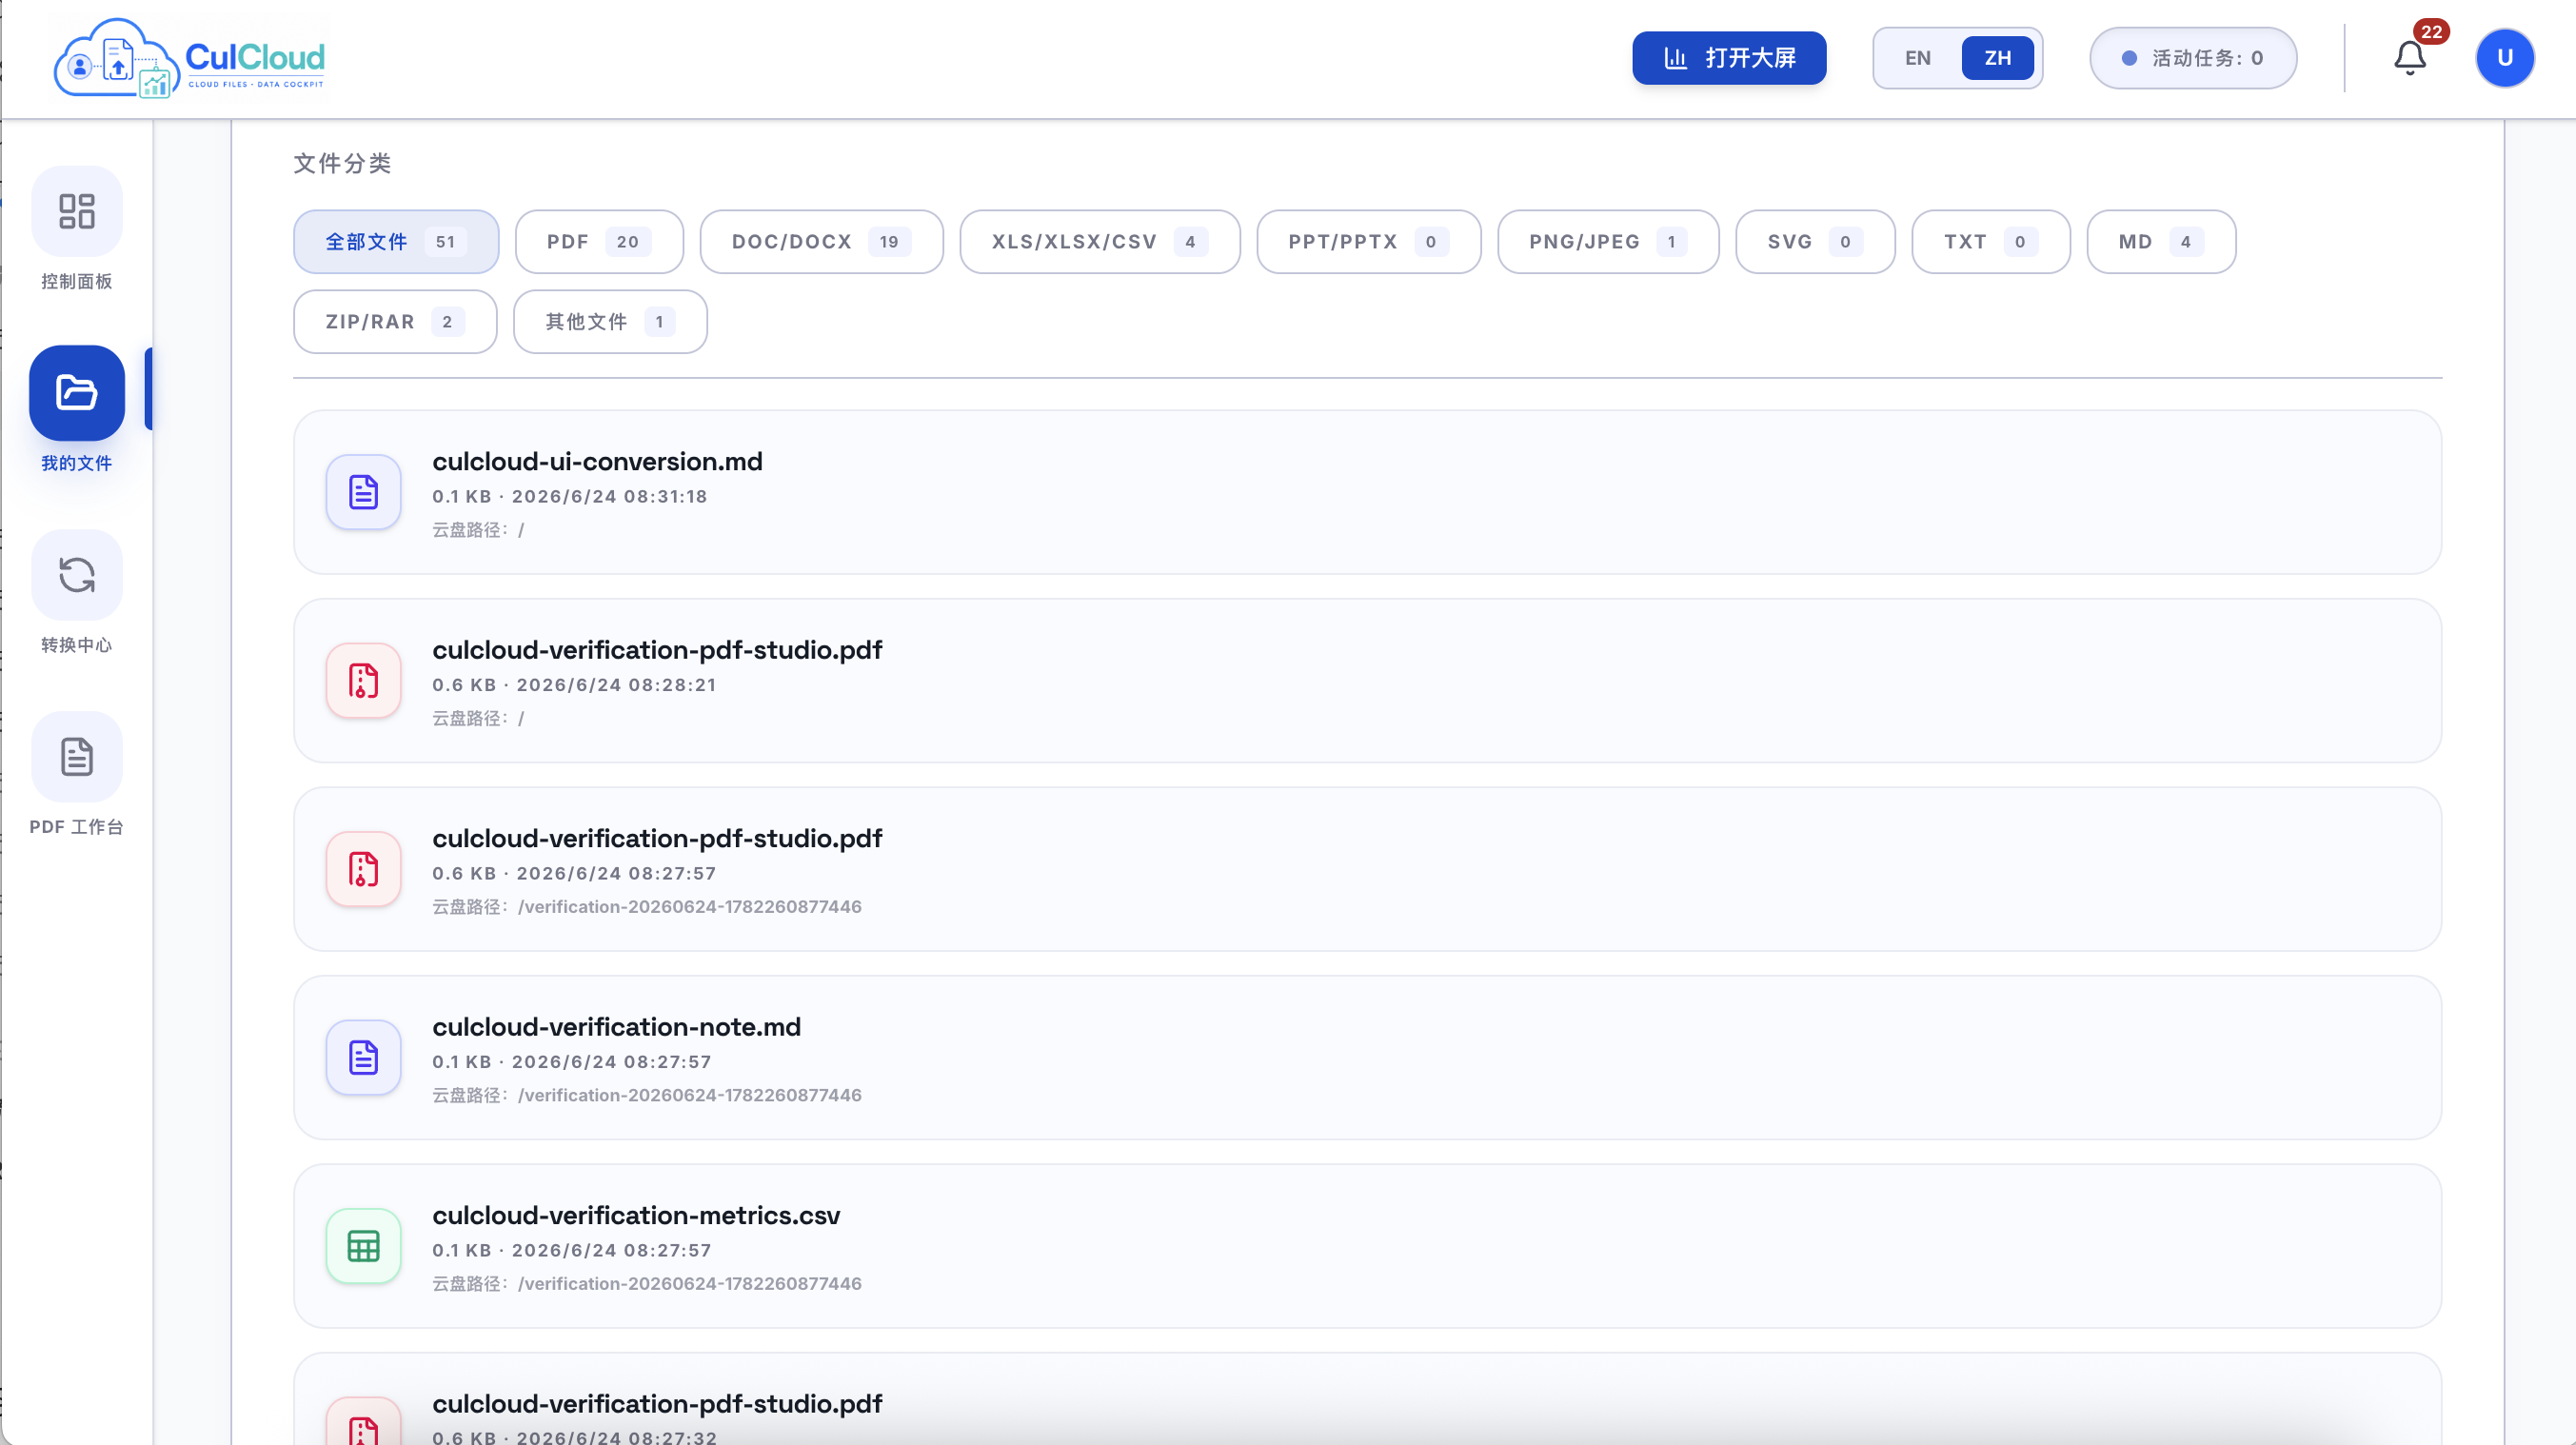
\includegraphics[width=\linewidth,height=0.25\textheight,keepaspectratio]{figures-png/ui/manual/fig05-manual-02-file-uploaded-list.png}
    \caption{上传后文件列表}
  \end{subfigure}
  \caption{文件管理模块界面结果图}
  \label{fig:chap05-file-manual-group}
\end{figure}

\section{文件预览模块的实现}

\subsection{预览类型识别}

文件预览由前端 \texttt{PreviewFrame} 和后端 \texttt{preview.py}、\texttt{services/preview.py} 协同实现。后端 \texttt{get\_preview\_metadata} 根据扩展名判断 \texttt{preview\_type}，并返回 \texttt{content\_url}。PDF、图片、音频和视频可直接通过内容接口返回；TXT 使用文本响应；Markdown 和 CSV 转换为隔离 HTML；Office 文件通过 Gotenberg 或转换服务生成 PDF 缓存。该设计使预览模块不要求前端理解所有文件解析细节，前端只需根据 \texttt{preview\_type} 选择对应展示组件。

预览接口分为元数据接口与内容接口两层。元数据接口负责说明文件是否可预览、预览类型和内容地址；内容接口负责返回字节流或渲染后的 HTML。这样做可以让前端先决定展示容器，再按需加载实际内容，避免大文件在列表阶段被提前读取。对于 Office 文件，缓存对象名由源文件信息计算得到，重复预览时优先复用缓存，减少转换服务压力。

第 4 章算法 \ref{alg:preview-dispatch} 已给出预览分派规则。本章关注其实现位置：扩展名识别、内容地址生成和不可预览状态由后端完成，前端只根据返回的 \texttt{preview\_type} 选择 PDF、图片、音视频、文本或 HTML 容器。

预览分派还承担异常兜底职责。若文件类型无法识别，接口应明确返回不可预览状态，而不是让前端反复尝试打开内容地址；若 Office 预览缓存生成失败，页面应保留下载入口和错误提示，避免用户误以为文件丢失；若 Markdown 或 CSV 内容较长，前端只负责展示后端生成的隔离内容，不把整份文本写入全局状态。这样可以把解析风险限制在预览模块内部。

缓存策略也影响用户体验。对于同一对象的重复预览，系统优先复用已生成的 PDF 或 HTML 缓存；当源文件发生移动或重命名时，内容接口仍应以对象名为准重新定位文件。该设计让预览模块既能减少转换服务压力，又能保持与文件管理模块的一致性。

\subsection{结构化内容渲染}

Markdown 和 CSV 的预览是该模块的关键实现。Markdown 需要在后端转换为 HTML，同时避免用户上传内容直接污染主页面；CSV 需要读取字节流、处理编码并生成表格化视图。图 \ref{fig:chap05-preview-manual-group} 展示了 PDF、Markdown 和 CSV 三类预览结果，三者分别对应二进制文档、标记文本和结构化表格。

从实现风险看，CSV 与 Markdown 预览比图片和 PDF 更容易出现编码、HTML 安全和长内容排版问题。因此后端采用独立响应内容承载渲染结果，前端通过预览框加载，既保留可读性，也减少对主页面状态树的影响。该策略适合课程资料中常见的配置文件、实验数据表和说明文档。

\begin{figure}[H]
  \centering
  \begin{subfigure}{0.32\textwidth}
    \centering
    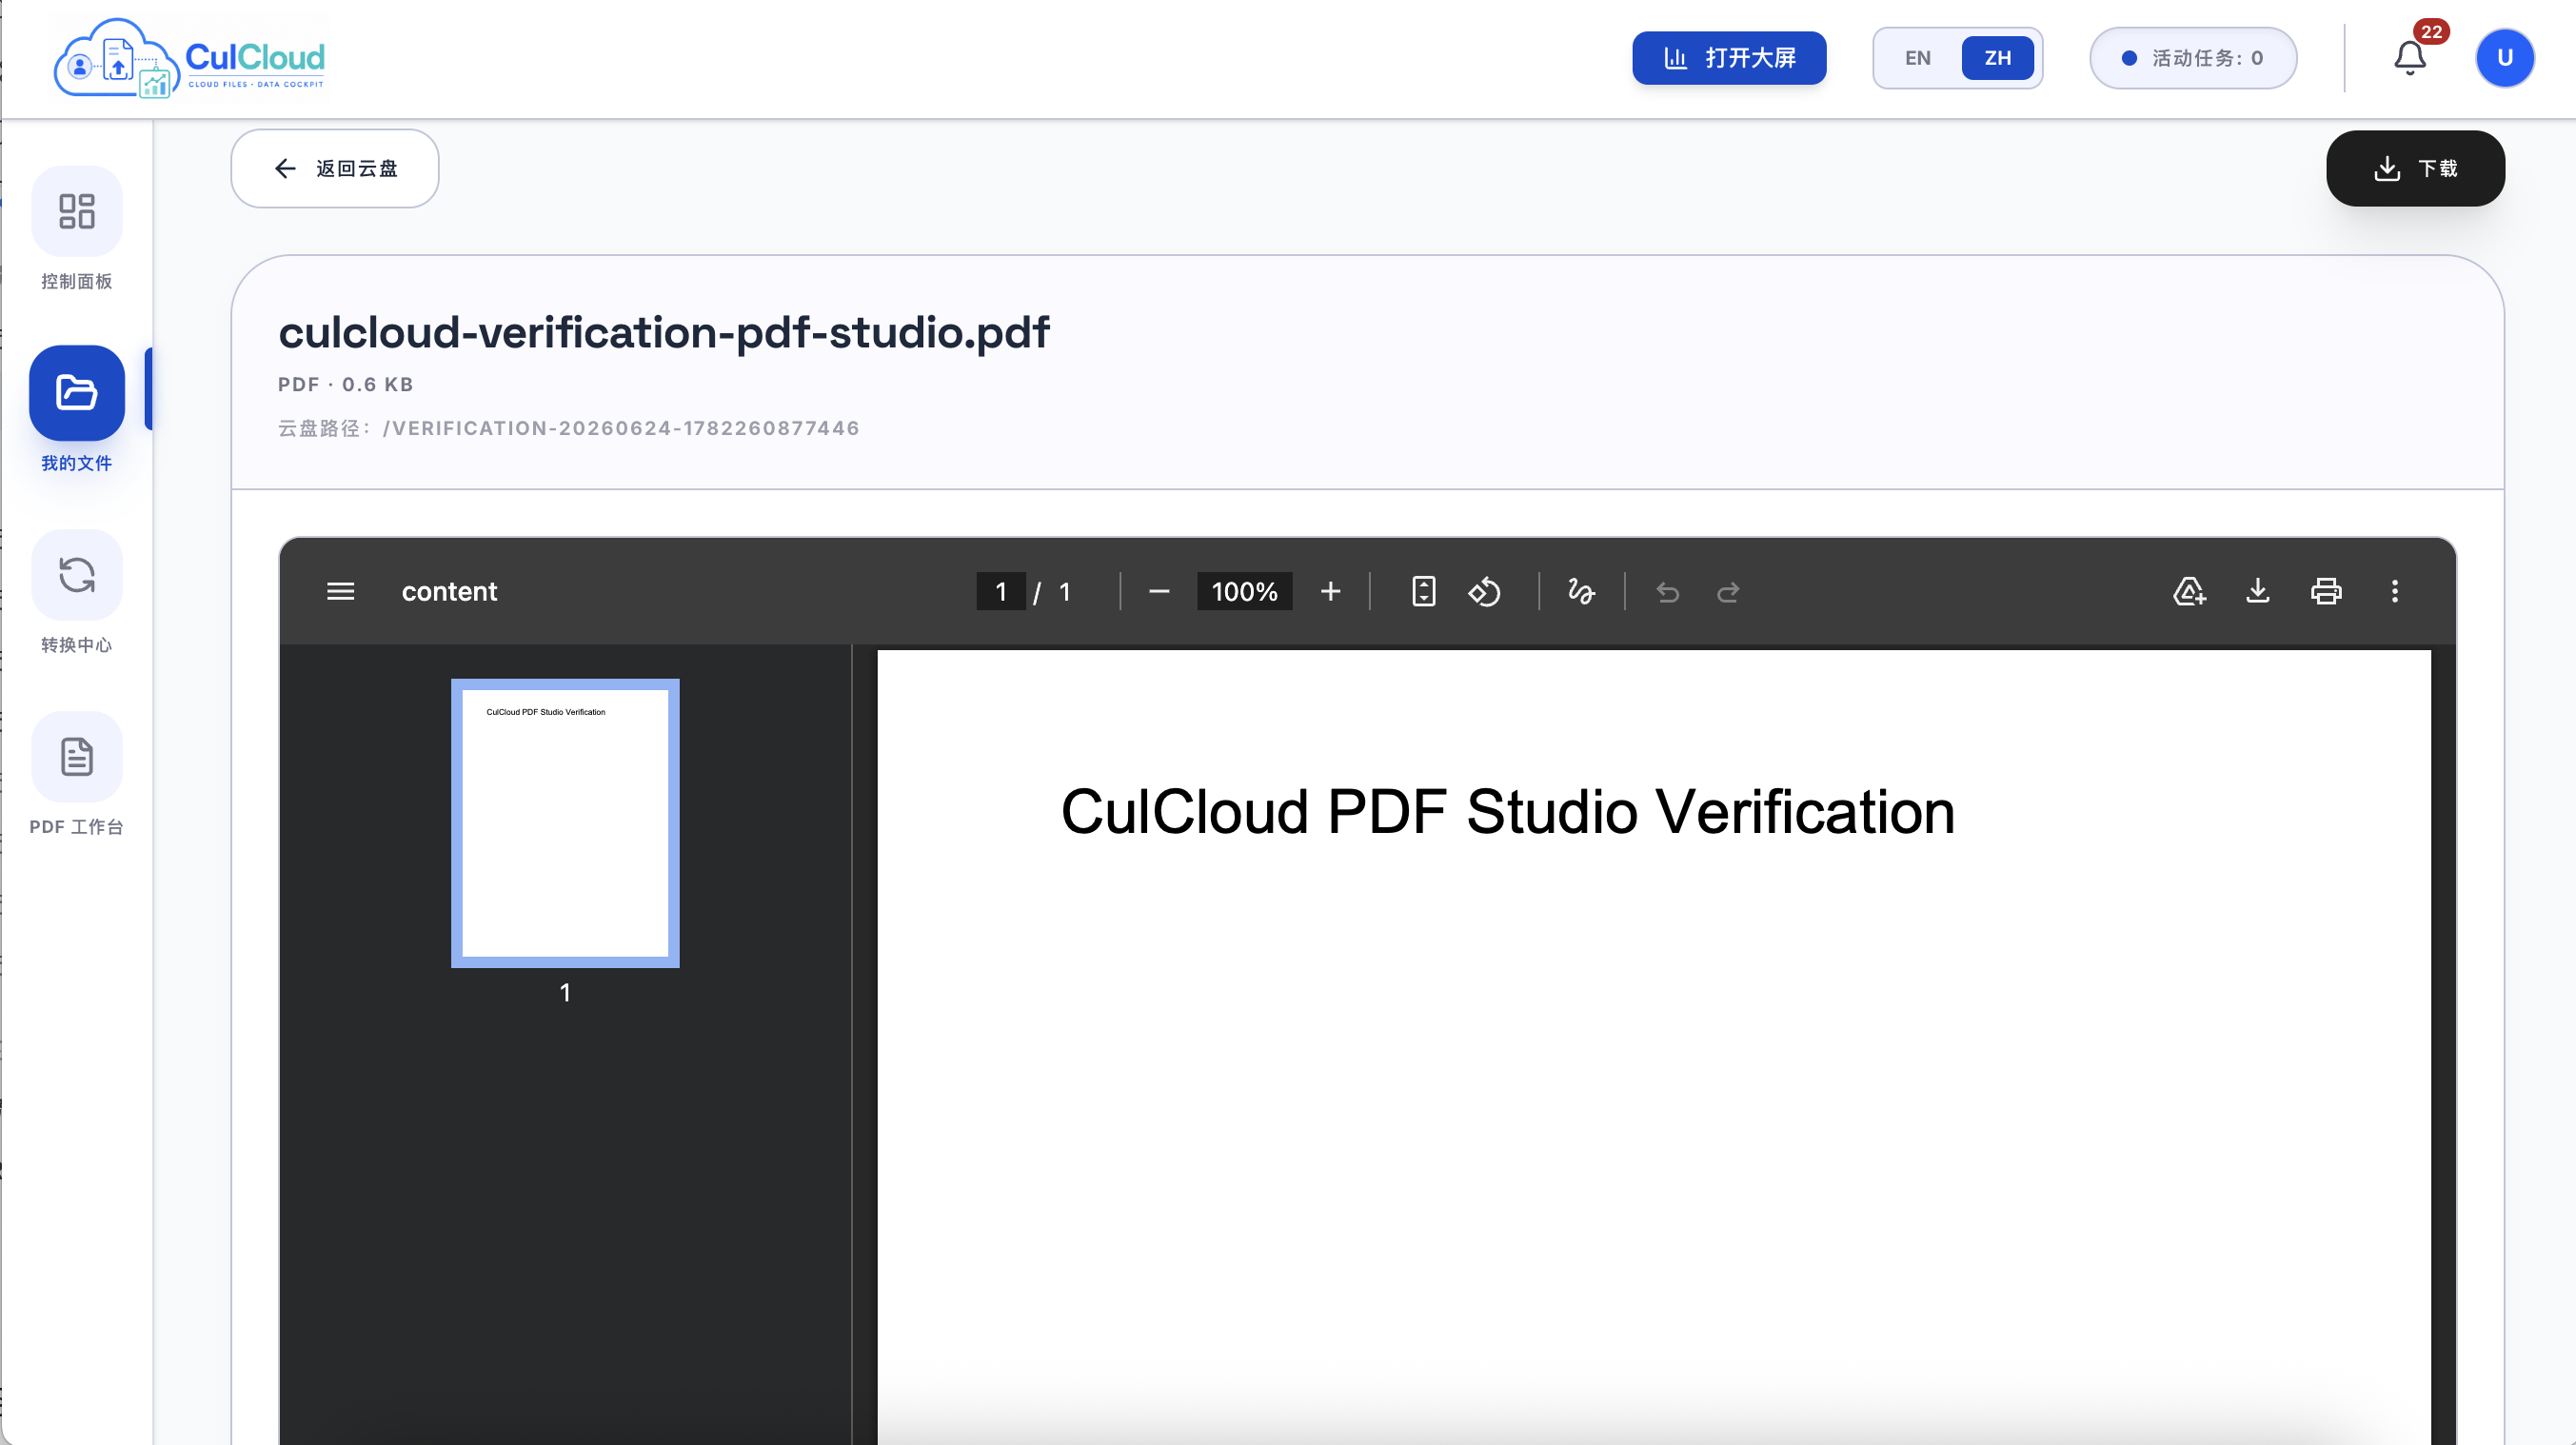
\includegraphics[width=\linewidth,height=0.20\textheight,keepaspectratio]{figures-png/ui/manual/fig05-manual-03-pdf-preview-result.png}
    \caption{PDF 预览}
  \end{subfigure}
  \hfill
  \begin{subfigure}{0.32\textwidth}
    \centering
    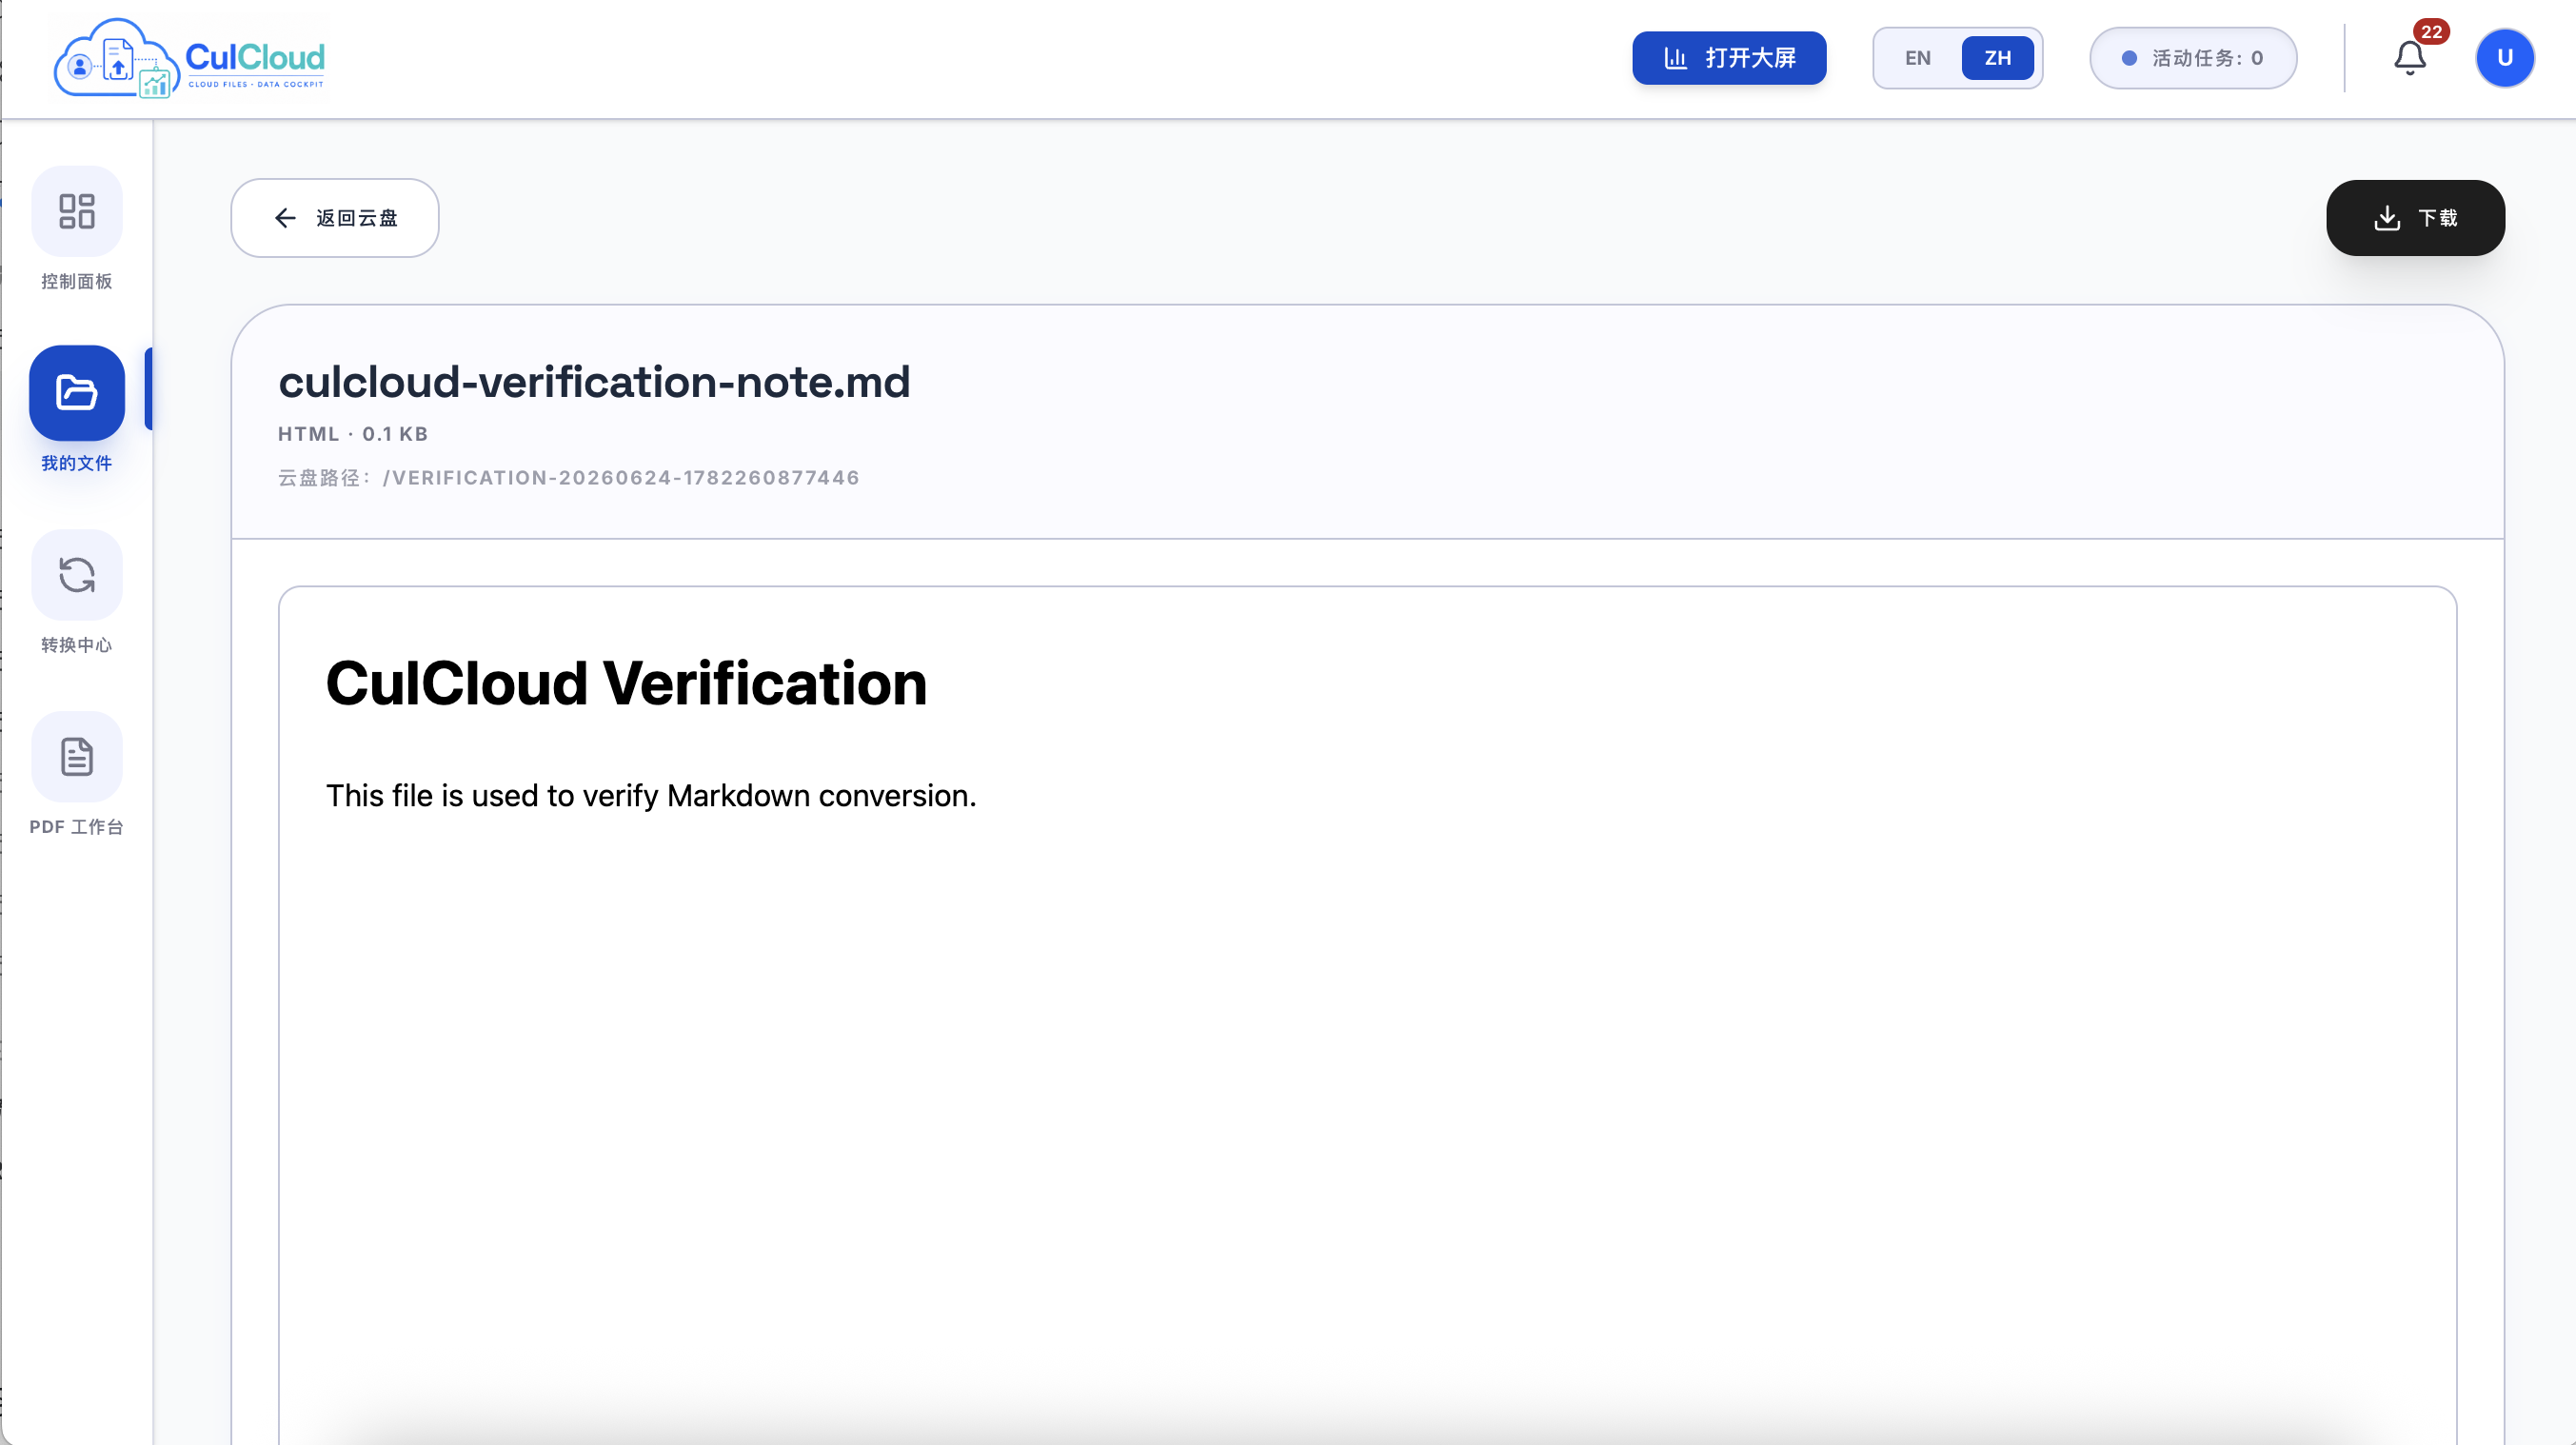
\includegraphics[width=\linewidth,height=0.20\textheight,keepaspectratio]{figures-png/ui/manual/fig05-manual-04-markdown-preview-result.png}
    \caption{Markdown 预览}
  \end{subfigure}
  \hfill
  \begin{subfigure}{0.32\textwidth}
    \centering
    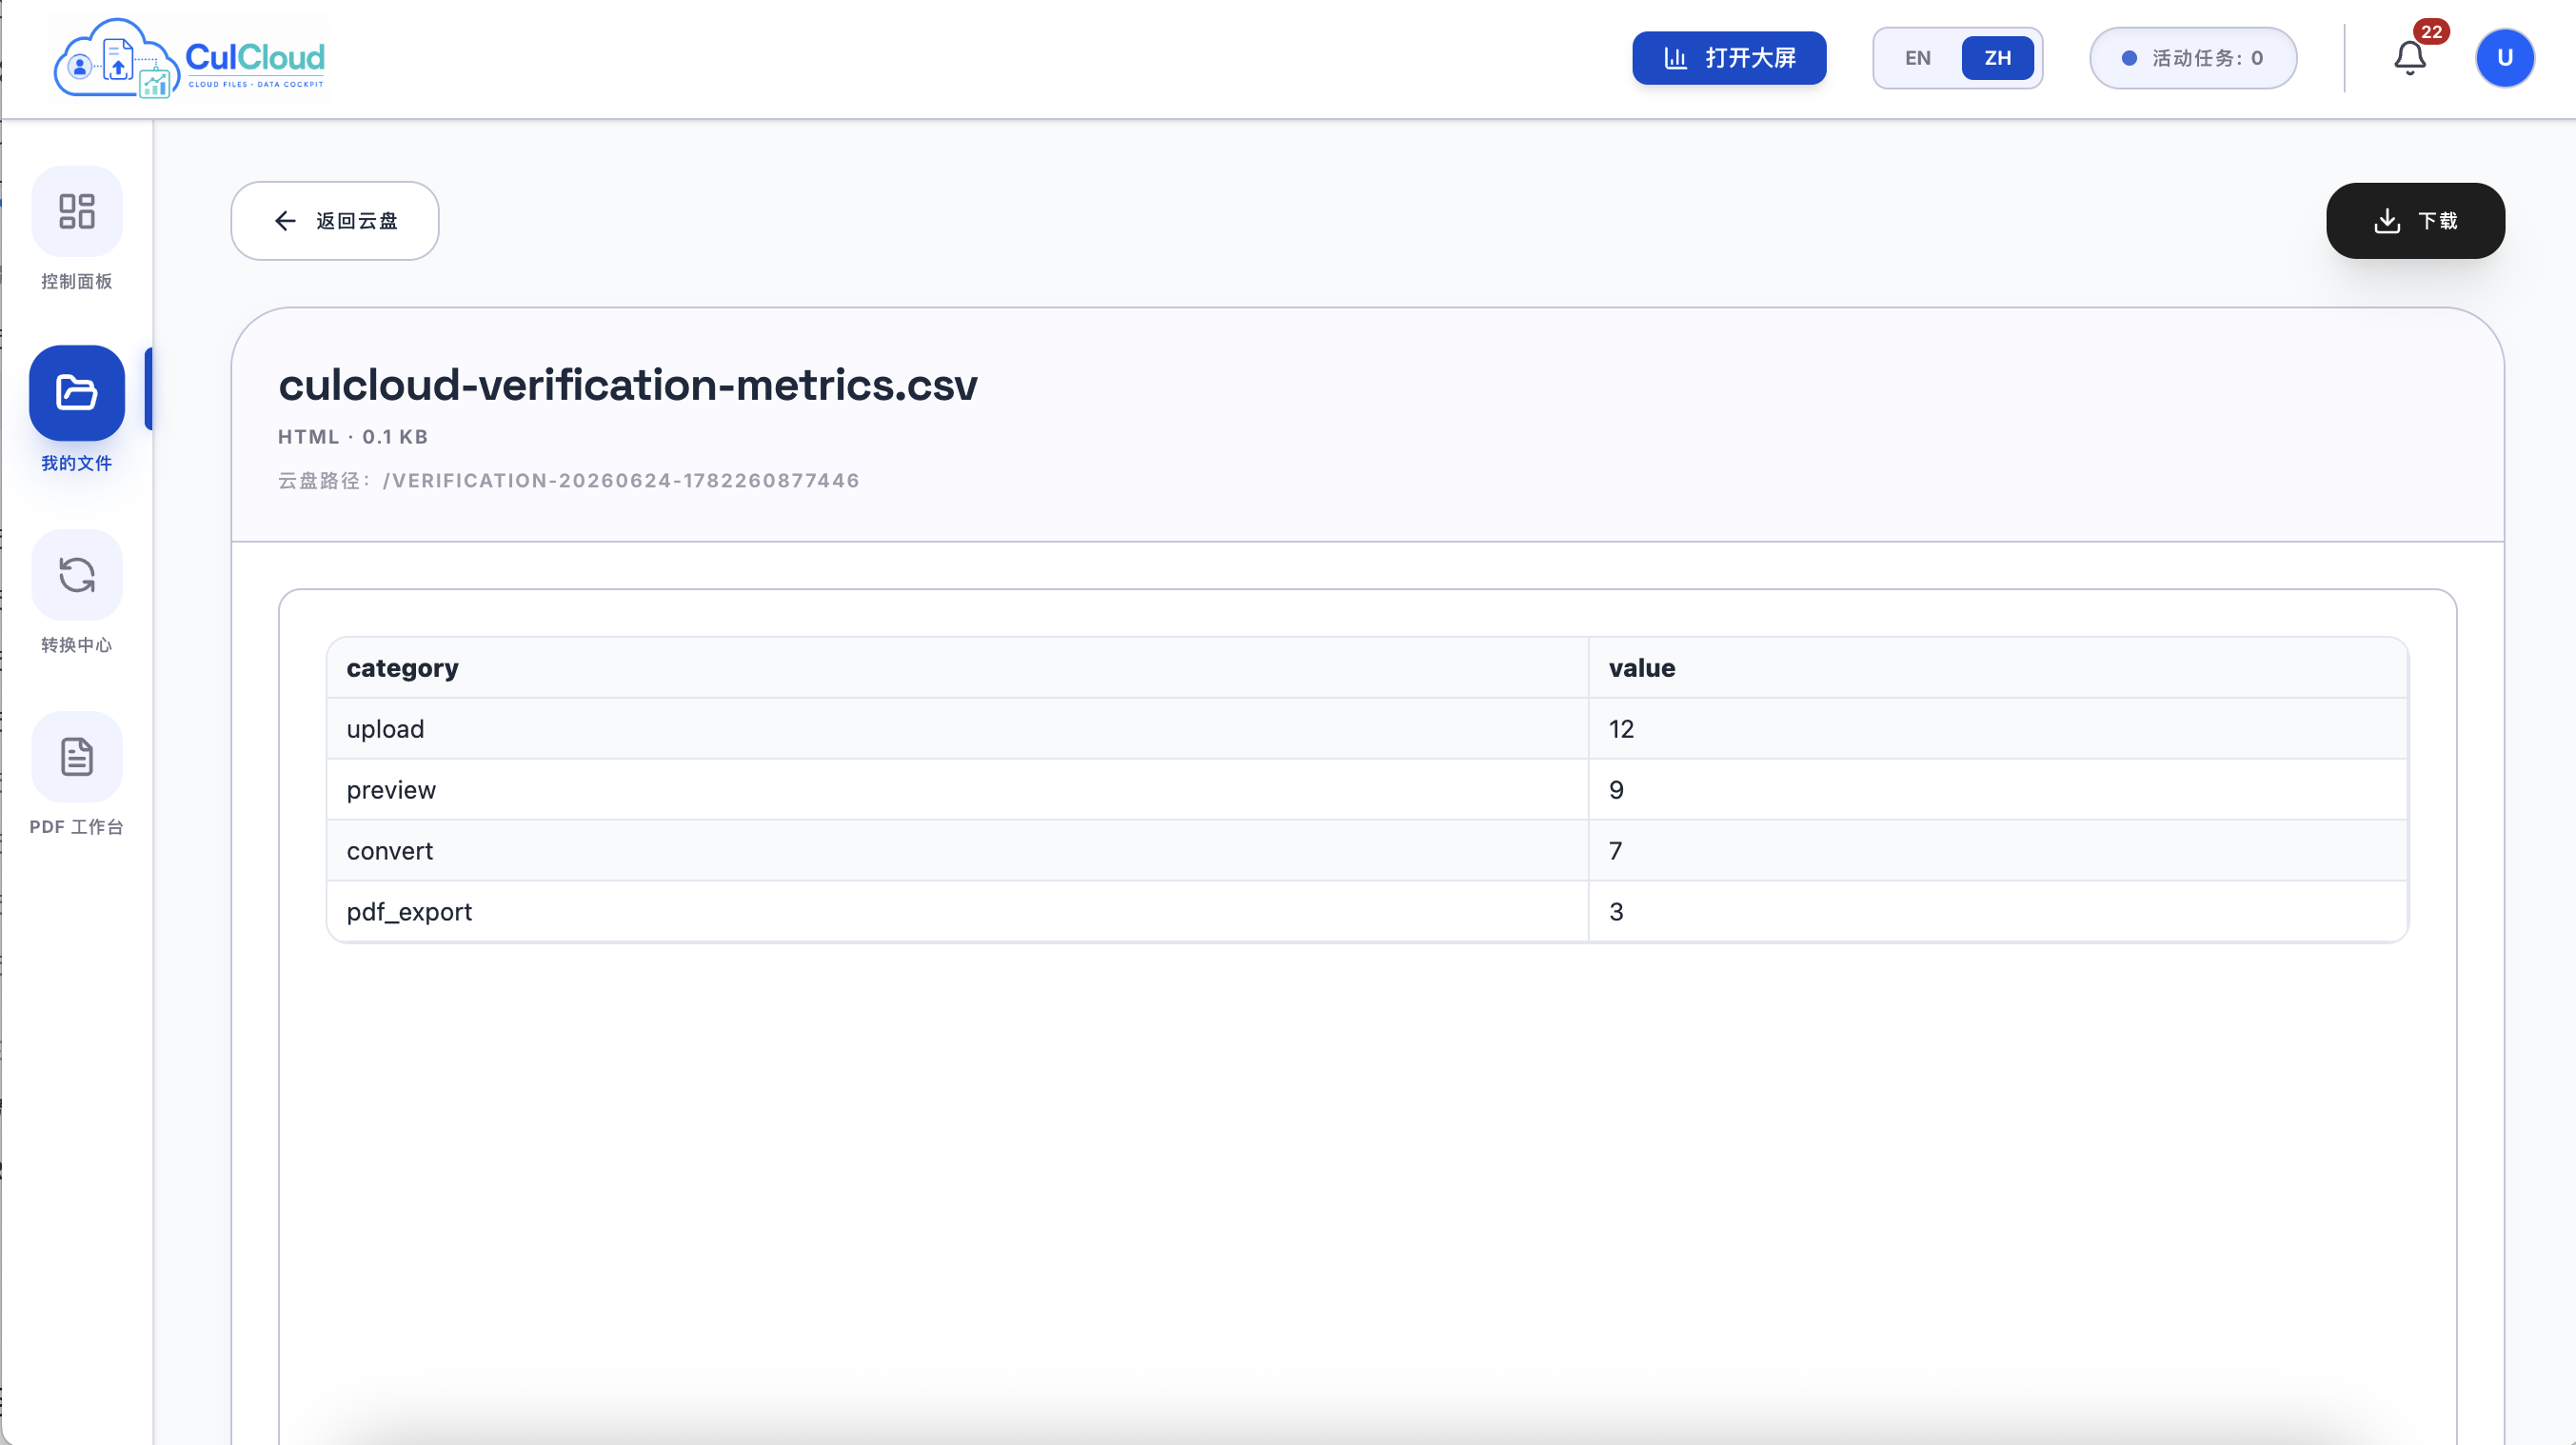
\includegraphics[width=\linewidth,height=0.20\textheight,keepaspectratio]{figures-png/ui/manual/fig05-manual-05-csv-preview-result.png}
    \caption{CSV 预览}
  \end{subfigure}
  \caption{文件预览模块界面结果图}
  \label{fig:chap05-preview-manual-group}
\end{figure}

\section{转换中心模块的实现}

\subsection{白名单与能力矩阵}

转换中心由 \texttt{ConvertCenter.tsx} 实现，后端对应 \texttt{routers/convert.py} 和 \texttt{services/converter.py}。系统在前后端都维护 P0 白名单：前端 \texttt{P0\_WHITELIST} 控制用户可选择的转换项，后端 \texttt{\_assert\_p0\_whitelist} 在 API 层再次拒绝未开放格式。这样即使前端被绕过，后端也不会执行未验证的转换路径。转换能力信息由 \texttt{/api/v1/convert/capabilities} 返回，便于前端按文件扩展名过滤目标格式。

白名单设计体现了系统的能力边界。项目并没有把所有库中理论可调用的转换函数都暴露给用户，而是只开放经过页面、接口和产物验证的高频链路。前端负责降低误操作概率，后端负责最终安全约束。该双层约束可以在后续扩展格式时逐项放开，而不会影响已经稳定的转换路径。

\subsection{异步任务执行}

转换任务提交后，后端调用 \texttt{set\_task\_status(task\_id, pending)} 写入初始状态，并通过 FastAPI BackgroundTasks 调用 \texttt{async\_convert\_task}。后台任务读取源文件，执行 \texttt{DocumentConverter} 中对应方法，例如 \texttt{word\_to\_pdf}、\texttt{csv\_to\_pdf}、\texttt{markdown\_to\_pdf}、\texttt{svg\_to\_png} 等。成功后，结果写入 MinIO 的 \texttt{conversions/} 前缀，任务状态更新为 \texttt{success} 并返回 API 代理下载地址；失败时写入 \texttt{failed} 与错误原因。图 \ref{fig:chap05-conversion-success} 展示了转换完成后的当前任务状态。

第 4 章算法 \ref{alg:async-task-process} 概括了转换与 PDF 导出共用的异步处理模式。代码实现中，转换中心对应 \texttt{async\_convert\_task}，PDF 编辑室对应 \texttt{async\_pdf\_process\_task}，二者都通过任务状态写入函数保持等待、处理中、成功和失败的一致语义。这样前端轮询、任务监控和管理驾驶舱读取到的是同一套状态来源。

前端轮询并不是无限循环，而是以第 4 章式 \ref{eq:polling-stop} 作为终止条件。\texttt{ConvertCenter.tsx} 和 \texttt{PDFStudio.tsx} 在读取到成功或失败终态后停止定时查询，避免任务已经结束后仍持续请求后端。

转换结果下载采用 API 代理地址，而不是直接暴露 MinIO 内部地址。这样可以避免浏览器跳转到对象存储端口后出现 Office 压缩包内部 XML 被直接打开等异常体验，也让下载行为继续受后端接口控制。任务状态轮询由前端定时触发，轮询终止条件是任务进入成功或失败终态，避免长期无意义请求。

\begin{figure}[H]
  \centering
  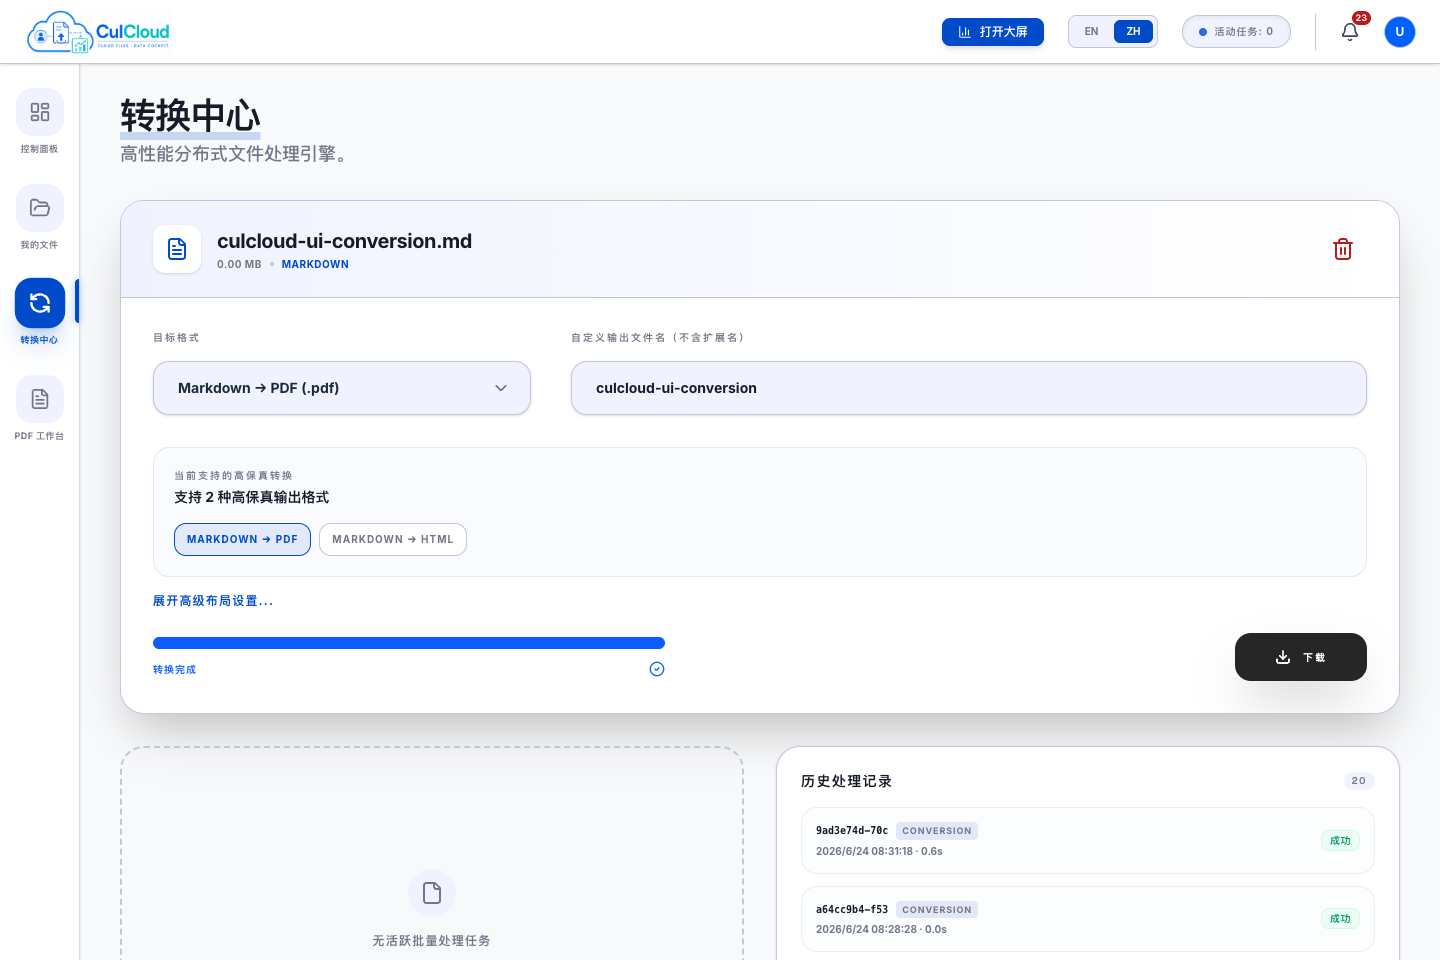
\includegraphics[width=0.92\textwidth,height=0.45\textheight,keepaspectratio]{figures-png/ui/fig05-10-conversion-current-success.png}
  \caption{转换中心任务完成界面结果图}
  \label{fig:chap05-conversion-success}
\end{figure}

\section{PDF 编辑室模块的实现}

\subsection{页面工作区}

PDF 编辑室由 \texttt{PDFStudio.tsx} 实现，核心状态包括 \texttt{WorkspacePage}、\texttt{Annotation}、当前工具、缩放比例和选中对象。用户选择 PDF 后，前端调用 \texttt{extractPdfPages}，后端使用 \texttt{DocumentConverter.pdf\_to\_images} 将每页转换为 PNG，并保存到 \texttt{previews/\{preview\_id\}/page\_N.png}。前端据此构建页面工作区，支持页面选择、排序、旋转、删除和批注。

PDF 工作区的设计采用“页面数组 + 批注数组”的状态模型。页面数组保存源对象、页码、旋转角度和尺寸信息，批注数组保存工具类型、坐标点、文本和颜色。排序与删除操作只改变页面数组，不直接修改源 PDF；导出时再由后端根据最终配置生成新文件。该方式使编辑过程可撤回、可重组，也避免频繁写入大体积 PDF 文件。

\subsection{批注与导出}

批注对象记录工具类型、坐标点、文本、颜色和线宽。导出时，前端将页面配置和批注数组提交给 \texttt{processPdf}，后端 \texttt{async\_pdf\_process\_task} 调用 \texttt{DocumentConverter.process\_pdf\_pages} 重组 PDF 并写入批注。图 \ref{fig:chap05-pdf-manual-group} 展示了 PDF 编辑工作区和导出后文件结果。该组图说明页面操作不是停留在浏览器状态，而是能够生成可打开的新 PDF 文件。

批注导出的难点在于坐标映射。前端操作发生在缩放后的画布上，后端写入发生在 PDF 页面坐标系中，因此导出配置必须携带前端画布宽高，并在后端按比例换算。对于文本批注，还需要加载适合中英文混排的字体，保证导出文件中的中文文本不会出现字符间距异常。

第 4 章式 \ref{eq:pdf-coordinate-map} 和算法 \ref{alg:pdf-export} 已给出坐标映射与导出规则。实现层面，前端提交页面配置数组和批注数组，后端在 \texttt{process\_pdf\_pages} 中读取源页面、应用旋转和顺序、换算批注坐标、加载 CJK 字体并写入新 PDF。这样 PDF 编辑室的交互状态能够转化为可打开的文件产物。

\begin{figure}[H]
  \centering
  \begin{subfigure}{0.48\textwidth}
    \centering
    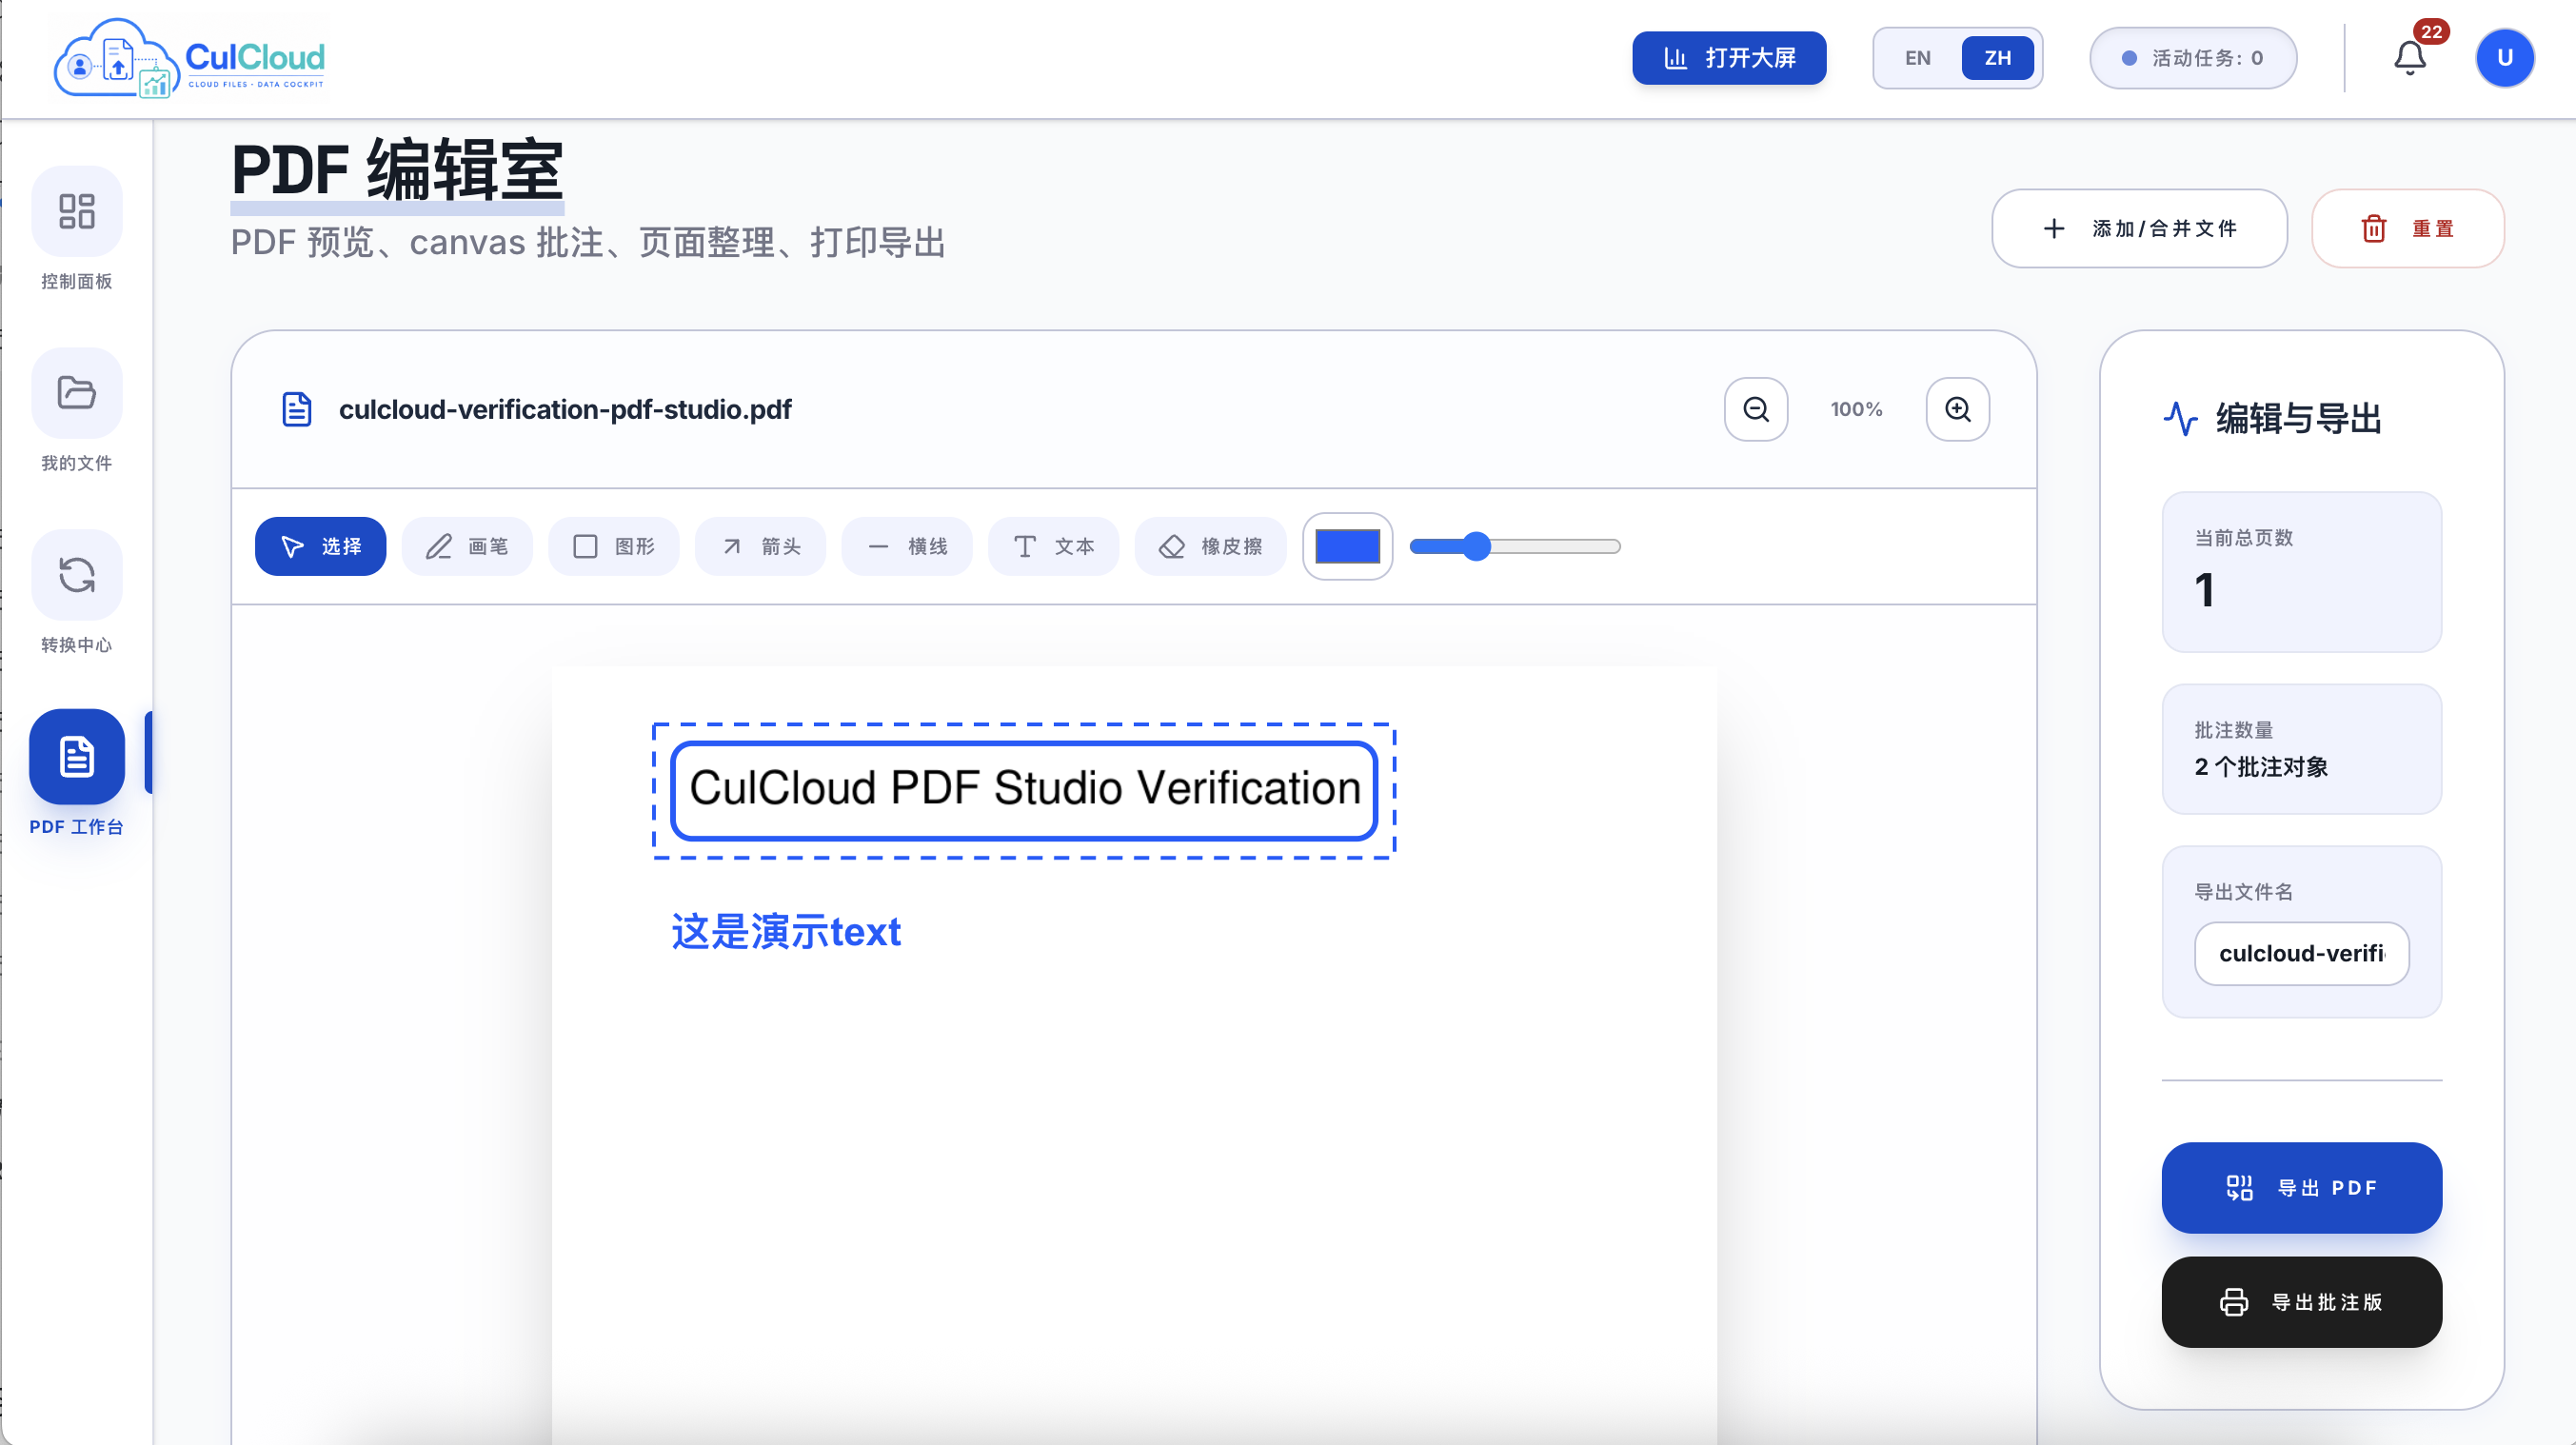
\includegraphics[width=\linewidth,height=0.25\textheight,keepaspectratio]{figures-png/ui/manual/fig05-manual-06-pdf-studio-annotation-workspace.png}
    \caption{页面与批注工作区}
  \end{subfigure}
  \hfill
  \begin{subfigure}{0.48\textwidth}
    \centering
    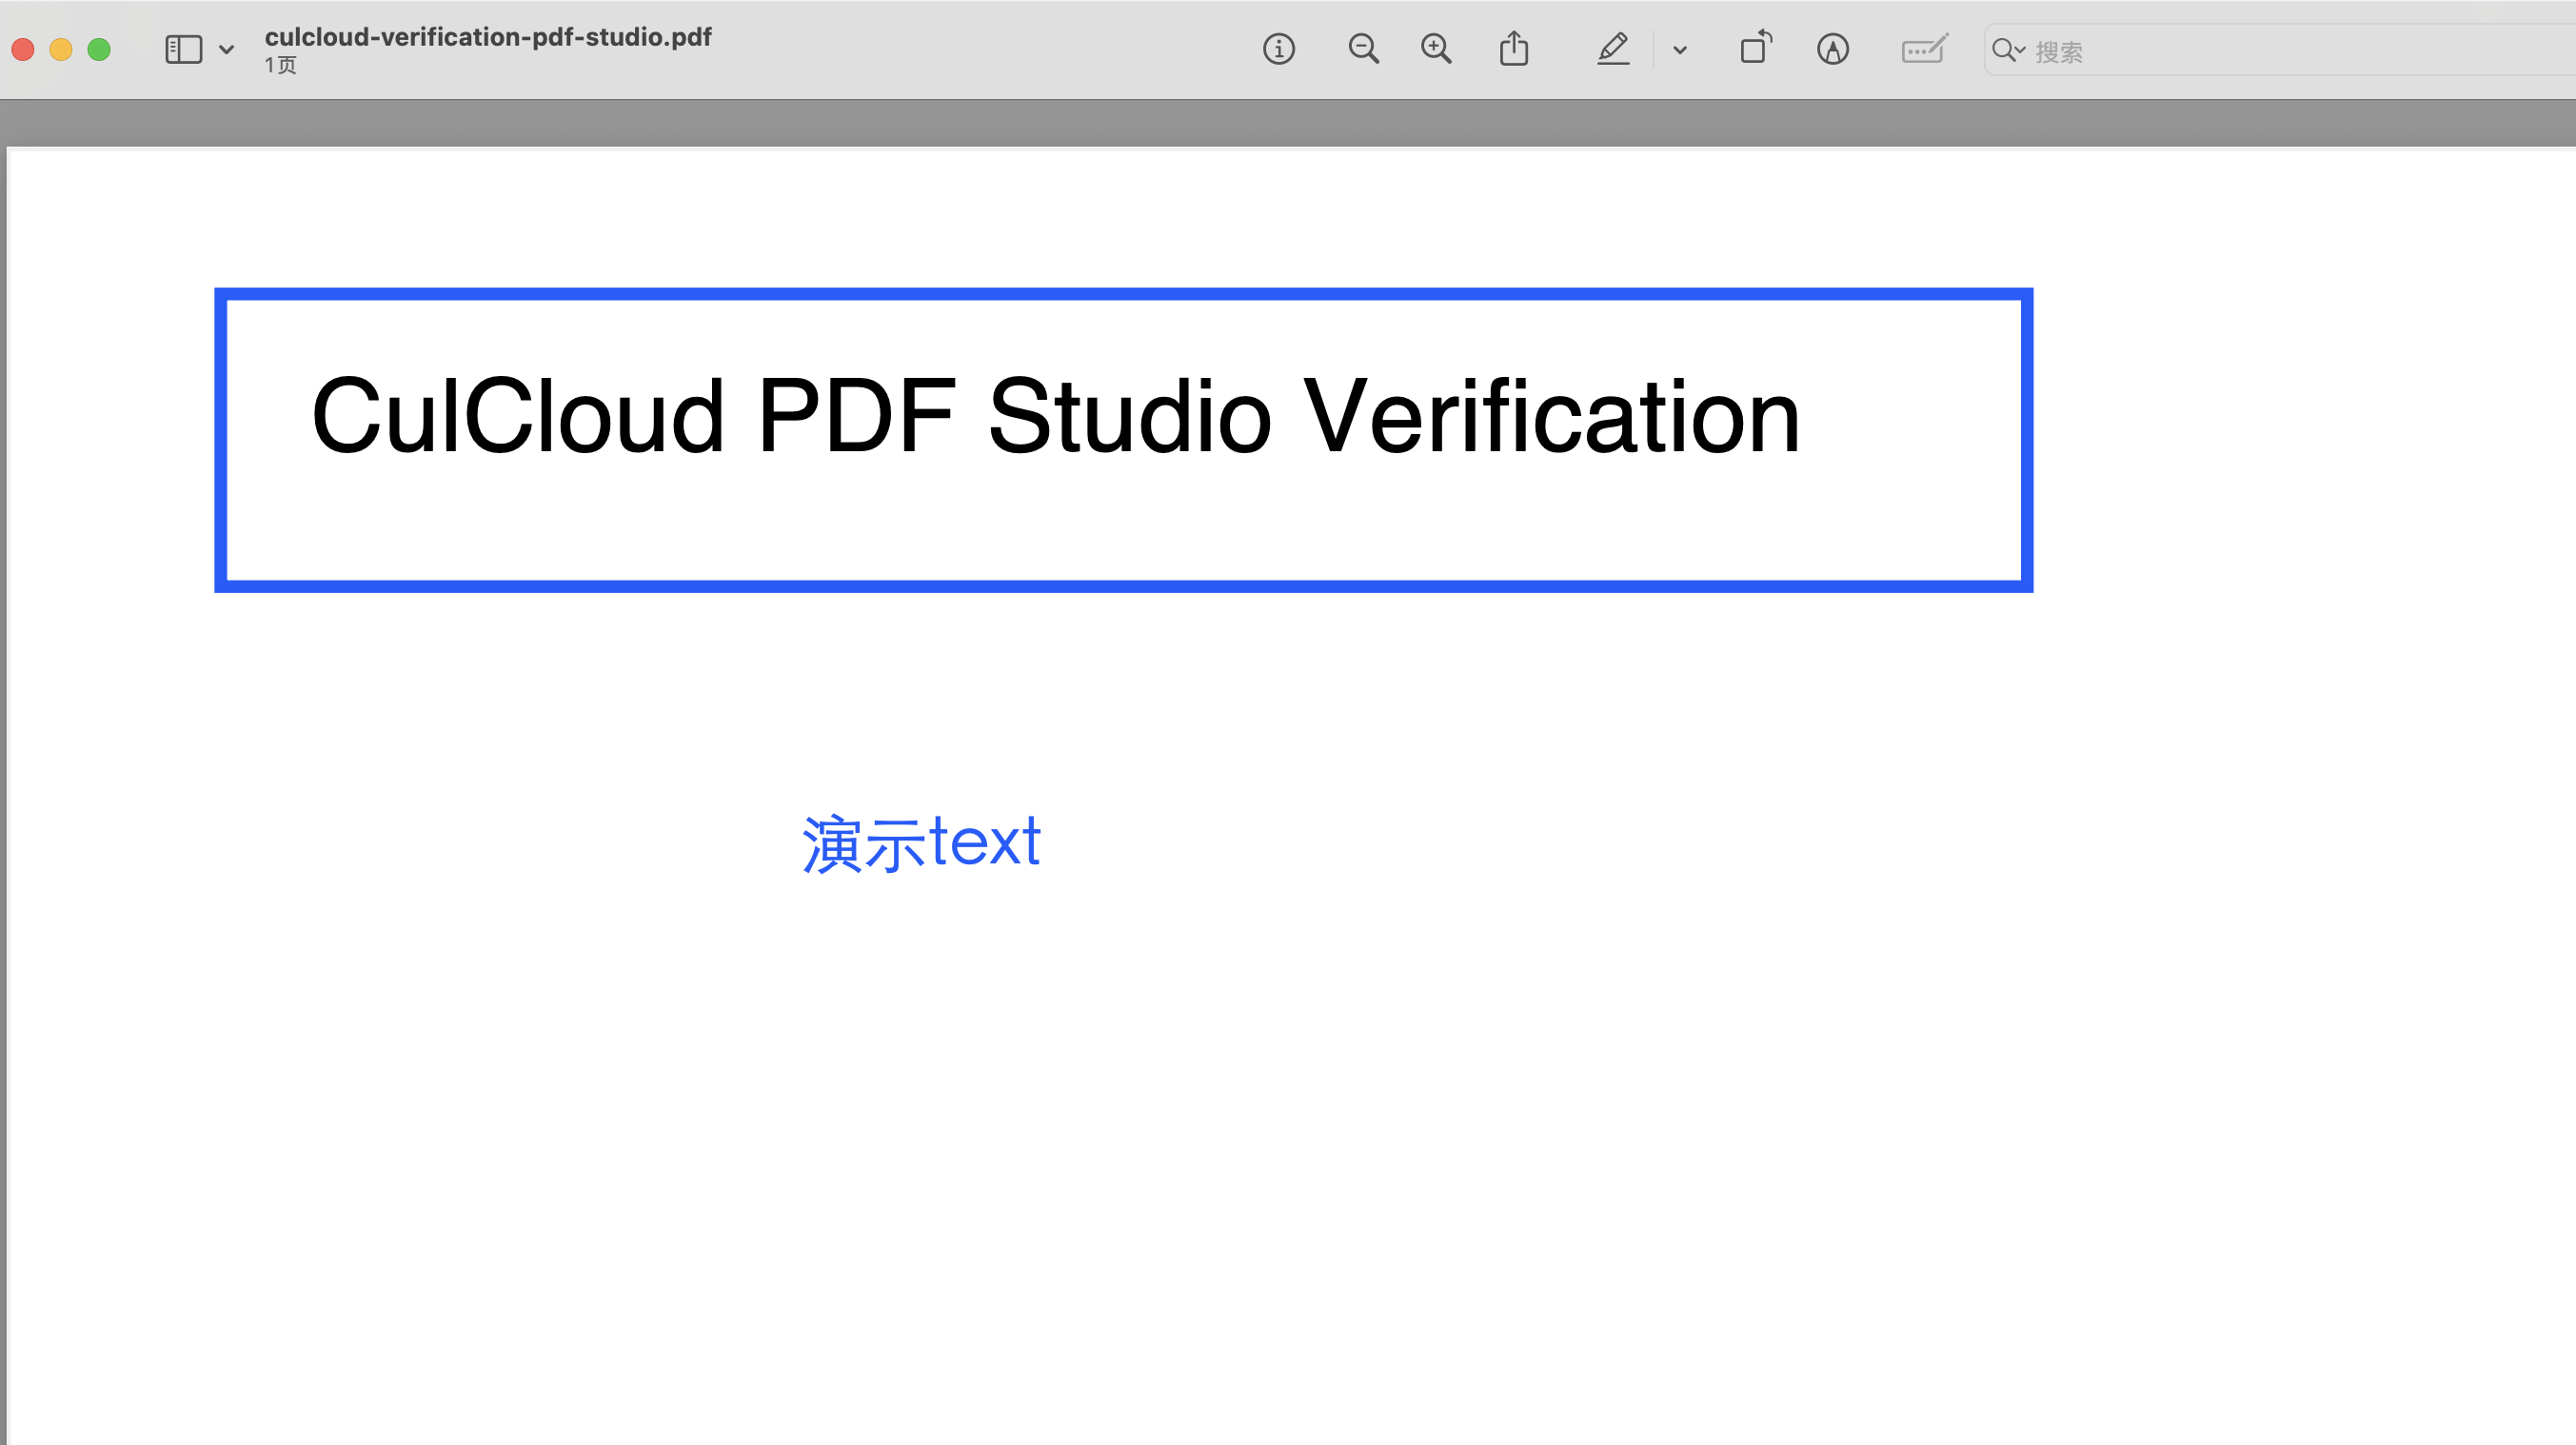
\includegraphics[width=\linewidth,height=0.25\textheight,keepaspectratio]{figures-png/ui/manual/fig05-manual-10-pdf-export-opened-result.png}
    \caption{导出后文件结果}
  \end{subfigure}
  \caption{PDF 编辑室处理结果图}
  \label{fig:chap05-pdf-manual-group}
\end{figure}

\section{管理驾驶舱模块的实现}

\subsection{实时运行视图}

管理驾驶舱由 \texttt{Analytics.tsx} 和 \texttt{AnalyticsSlides.tsx} 实现。第一屏通过 \texttt{useBizData} 直接读取 FastAPI 的实时接口，包括 \texttt{/api/v1/files}、\texttt{/api/v1/tasks/stats}、\texttt{/api/v1/tasks/queue-length}、\texttt{/api/v1/logs/timeline}、\texttt{/api/v1/logs/stats} 和 \texttt{/api/v1/system/health}。这些数值会随用户端上传、转换、PDF 导出和日志写入而变化，是系统当前运行状态。

第一屏的实现目标是反映“现在系统发生了什么”。文件数量来自当前 MinIO 对象，任务成功率来自 Redis 任务统计，近期事件来自日志时间线，服务状态来自健康检查快照。用户端完成一次文件转换后，任务统计和事件列表应随轮询刷新而变化，这也是管理端与用户端互通的关键证据。

\subsection{历史分析视图}

第二屏和第三屏读取 Flask Analytics 提供的历史分析接口。Flask 服务从 \texttt{data/spark-output/*.json} 读取 Spark 聚合结果，包含历史文件样本、历史转换任务、历史文件类型分布、历史转换桑基图、历史有效遥测、历史数据质量、历史存储水位和历史错误热力图。该部分用于体现大数据分析链路，不与第一屏实时指标混用。

历史分析视图的价值在于展示离线聚合能力。Spark 脚本对遥测样本执行文件格式分布、转换矩阵、访问趋势、质量报告和错误热力图统计，Flask 只负责把聚合结果转成 API。由于历史样本与实时业务数据不是同一口径，页面标题和正文均明确标注“历史”，避免将样本规模误解为当前运行规模。

\begin{figure}[H]
  \centering
  \begin{subfigure}{0.32\textwidth}
    \centering
    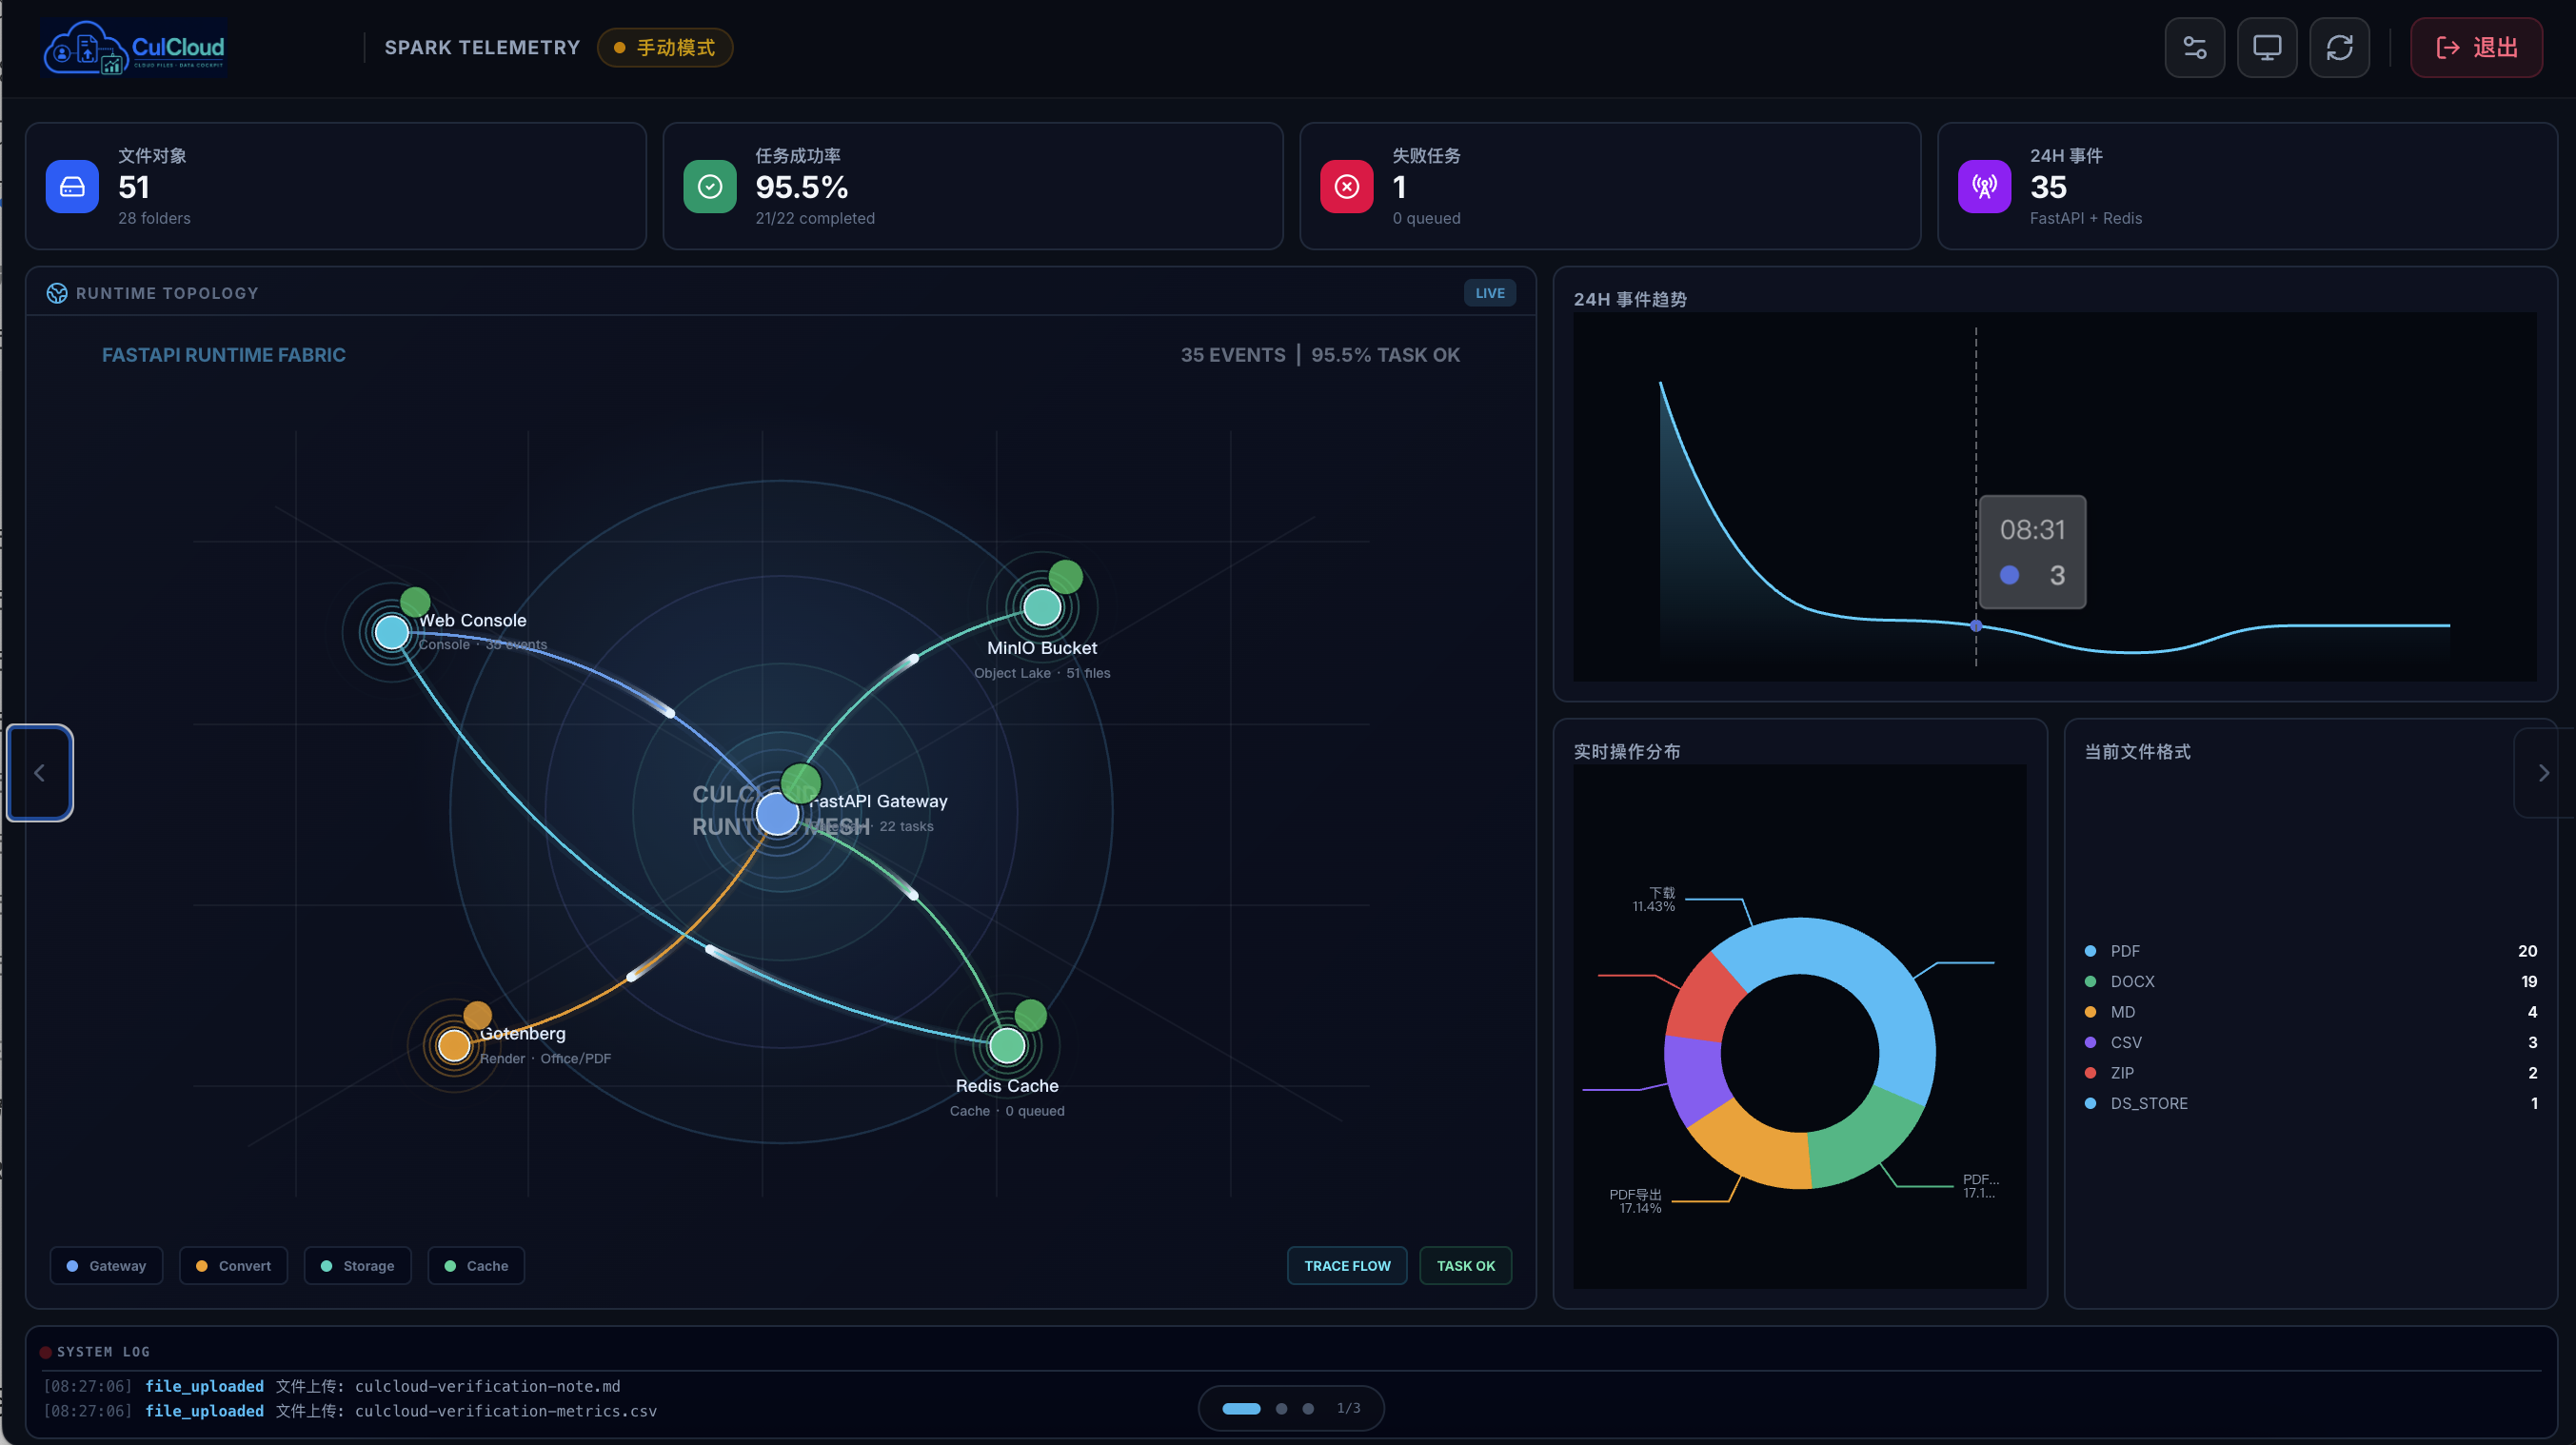
\includegraphics[width=\linewidth,height=0.20\textheight,keepaspectratio]{figures-png/ui/manual/fig05-manual-09-admin-runtime-topology-events.png}
    \caption{实时拓扑与事件}
  \end{subfigure}
  \hfill
  \begin{subfigure}{0.32\textwidth}
    \centering
    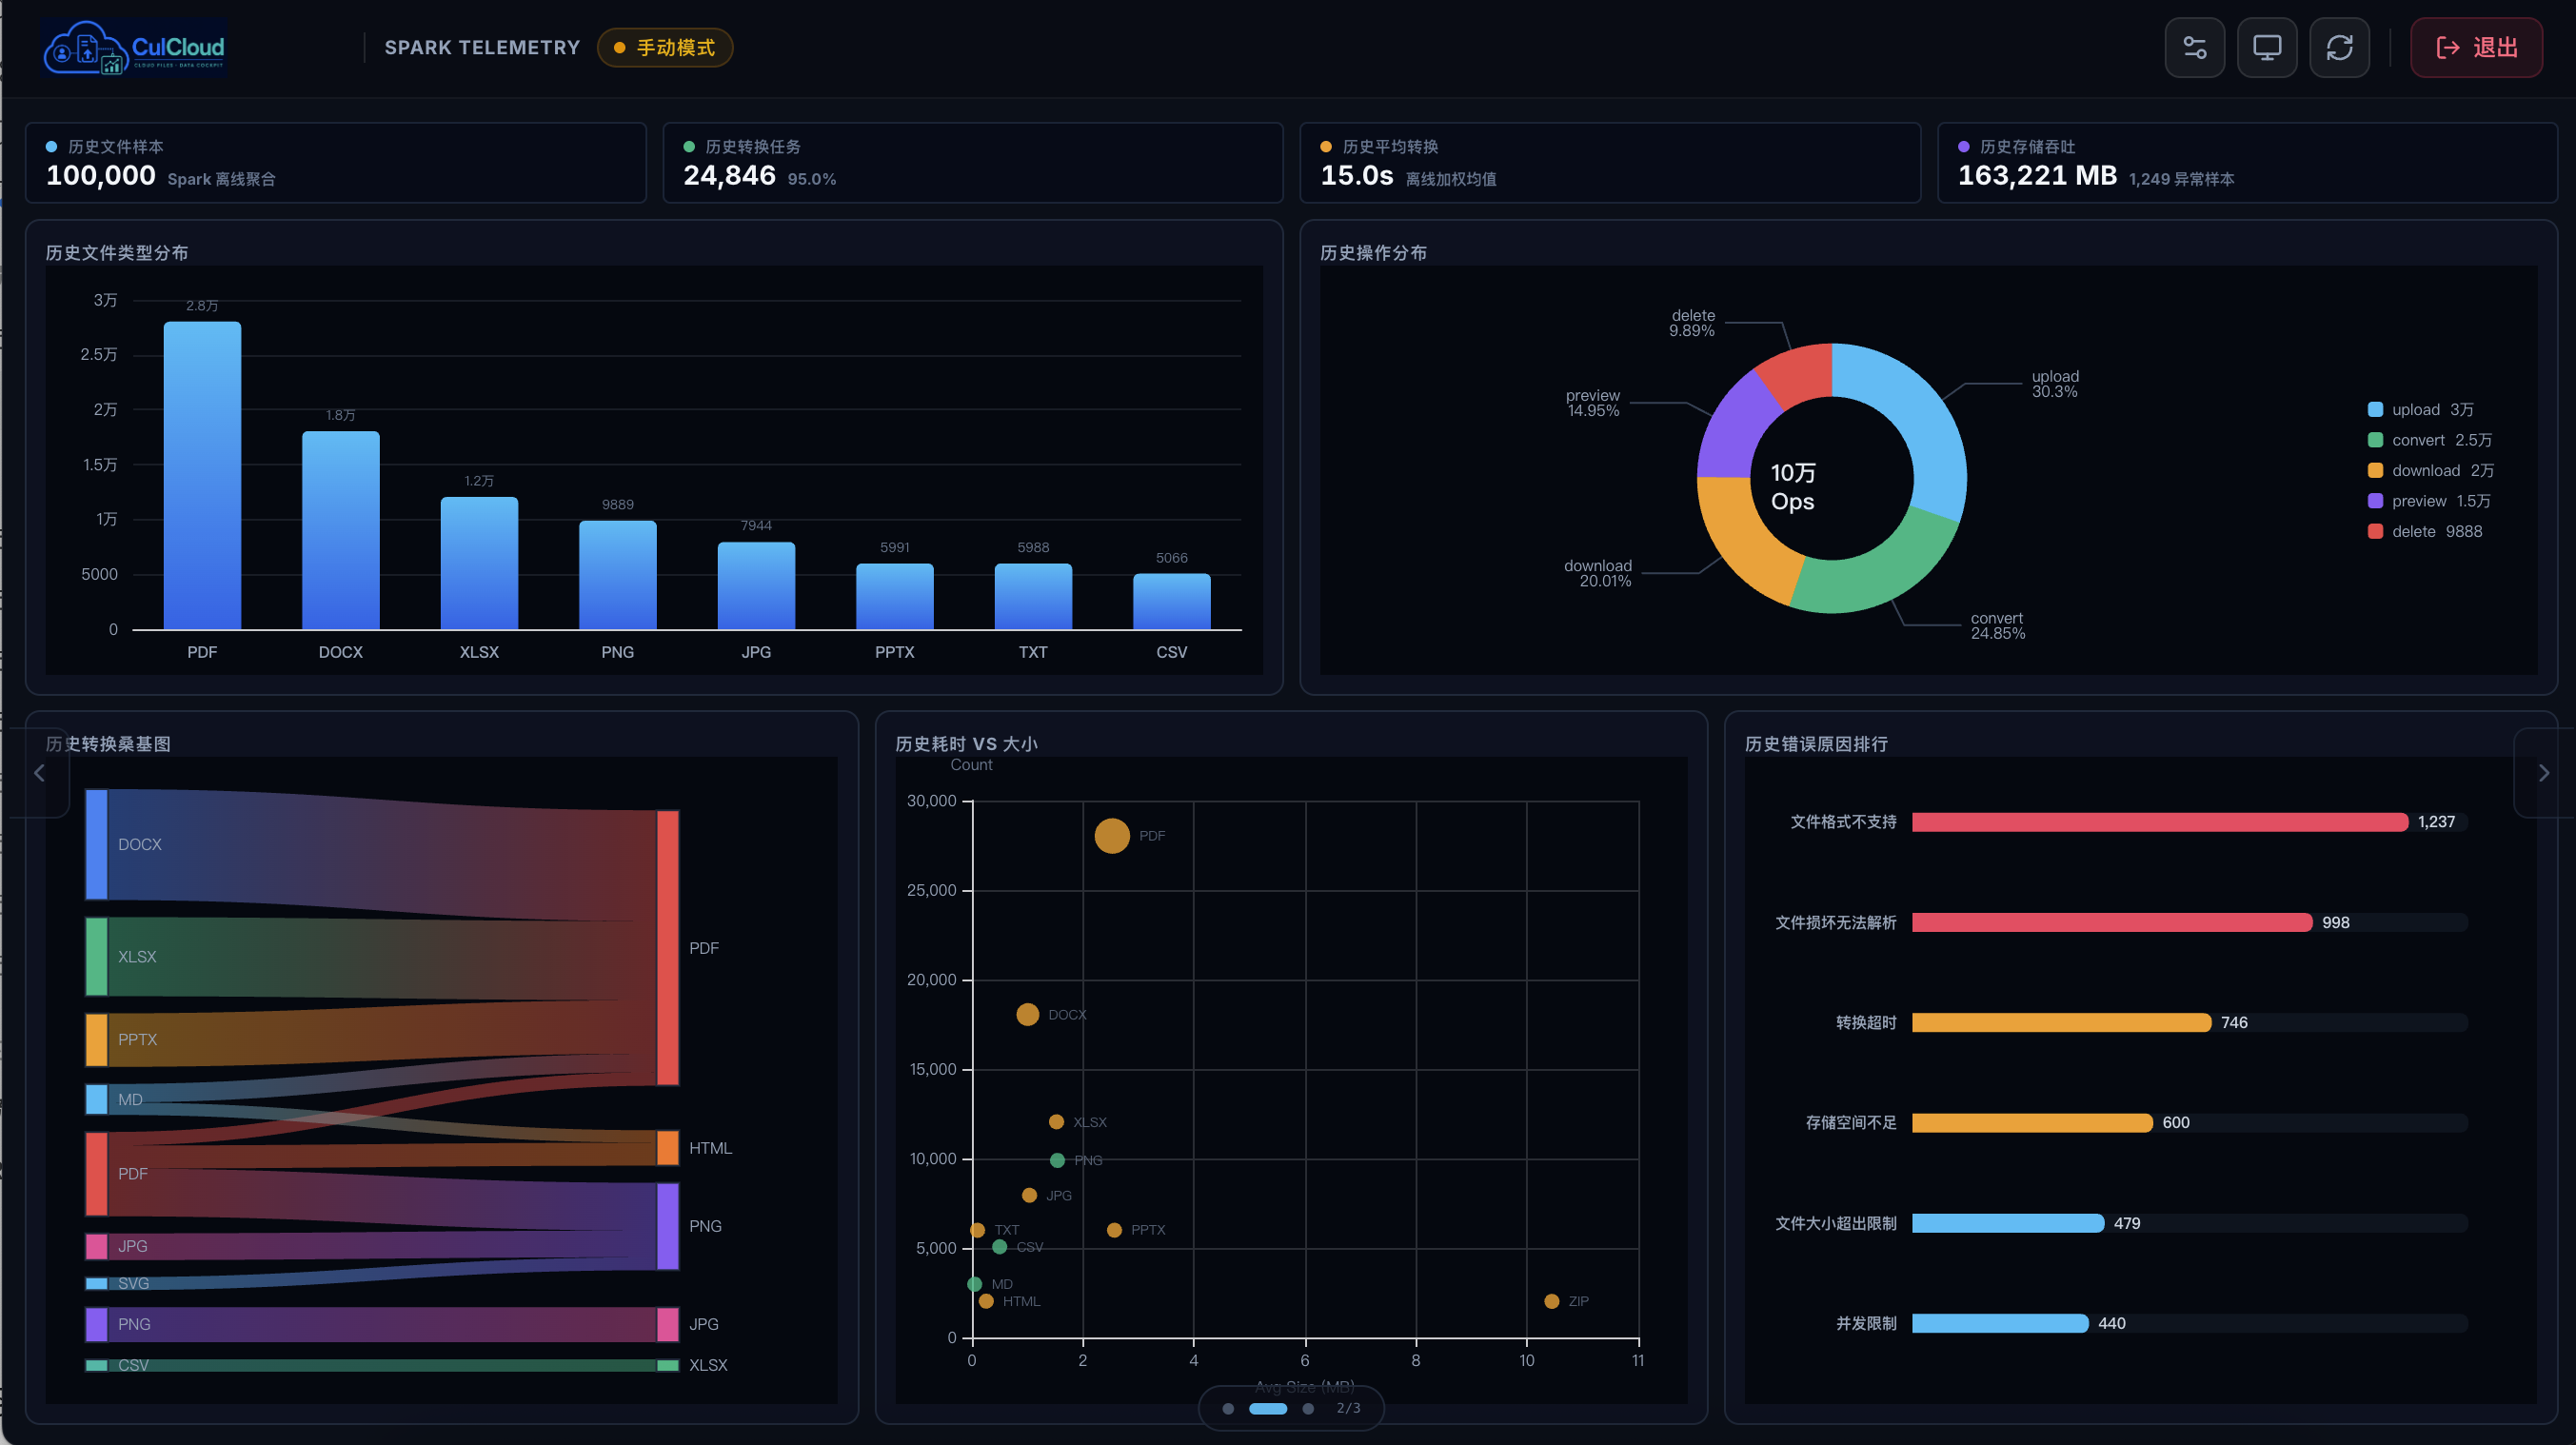
\includegraphics[width=\linewidth,height=0.20\textheight,keepaspectratio]{figures-png/ui/manual/fig05-manual-08-admin-historical-processing.png}
    \caption{历史转换分析}
  \end{subfigure}
  \hfill
  \begin{subfigure}{0.32\textwidth}
    \centering
    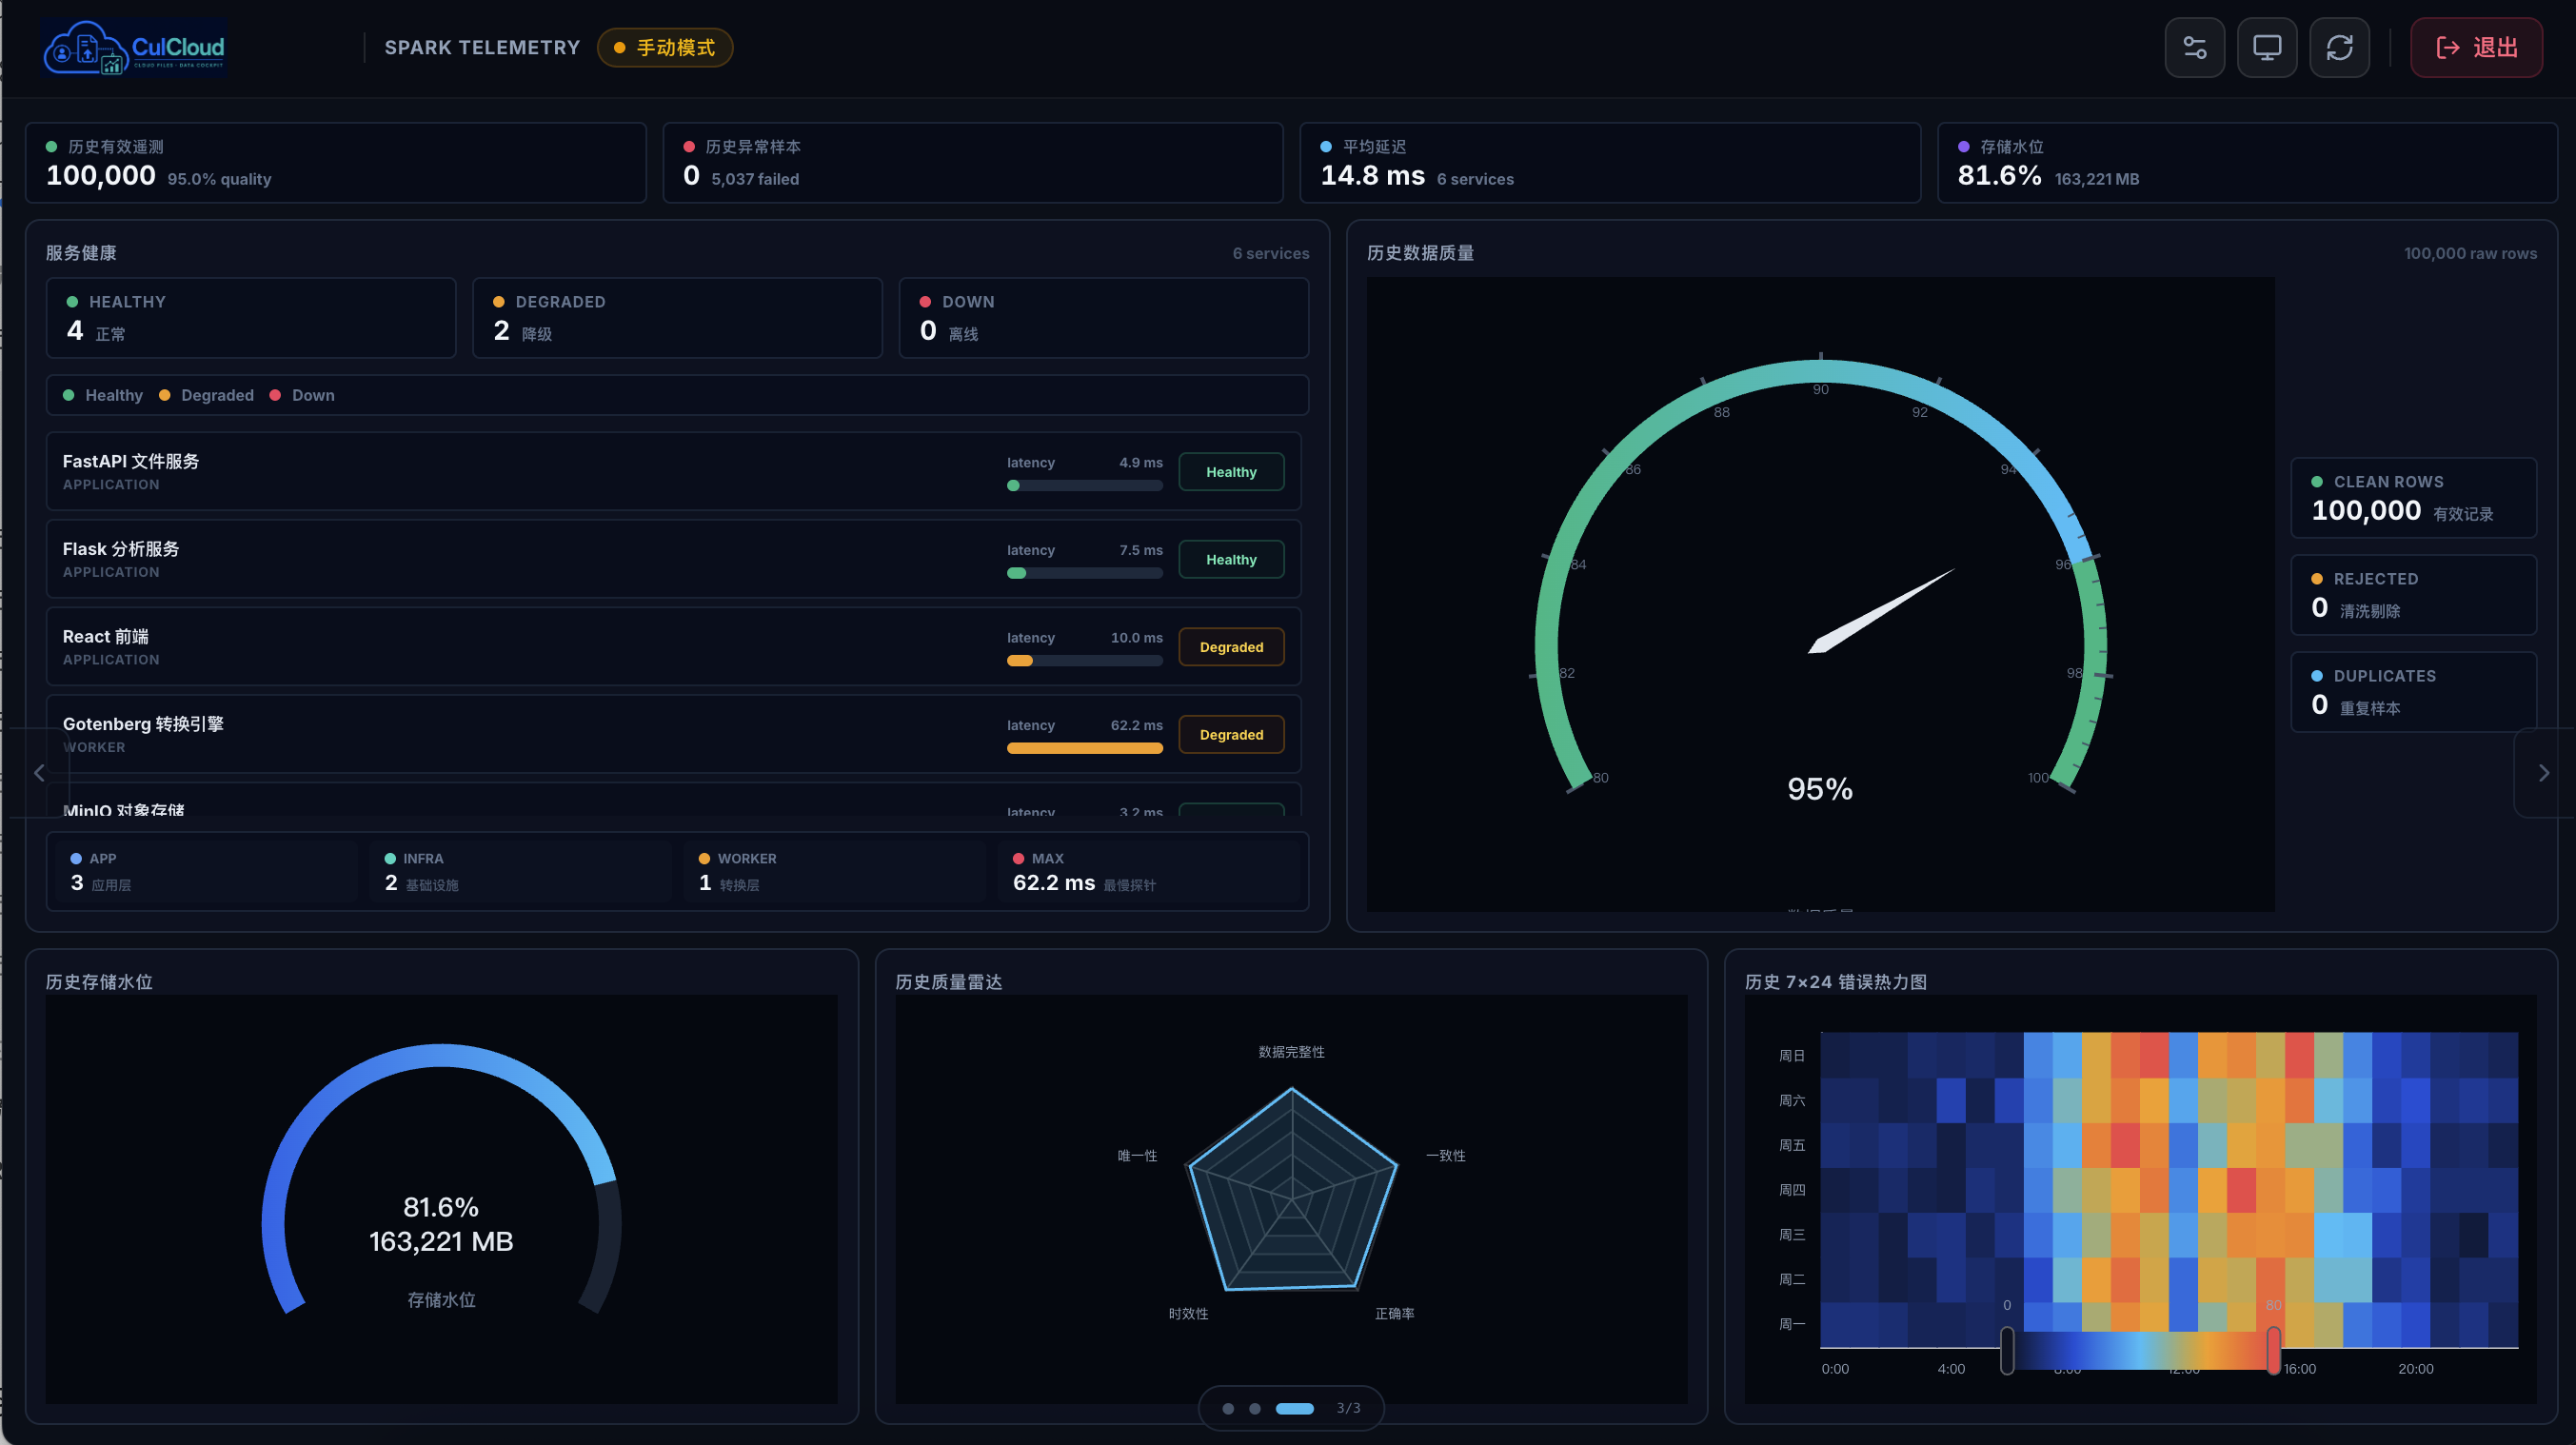
\includegraphics[width=\linewidth,height=0.20\textheight,keepaspectratio]{figures-png/ui/manual/fig05-manual-07-admin-historical-quality.png}
    \caption{历史质量分析}
  \end{subfigure}
  \caption{管理驾驶舱运行与历史分析结果图}
  \label{fig:chap05-admin-manual-group}
\end{figure}

\section{本章小结}

本章围绕真实代码位置说明了个人首页、我的文件、文件预览、转换中心、PDF 编辑室和管理驾驶舱的实现方式。系统实现的核心特点是前端视图、API 客户端、后端路由、领域服务、MinIO 对象和 Redis 状态之间形成清晰链路，使用户端操作能够产生可查询任务、可下载产物和管理端可观察数据。
